
\section{Langkah-Langkah Percobaan}
\subsection{Konfigurasi Router VPN PPTP PC dengan Router}

\begin{enumerate}

    \item Akses router melalui Winbox menggunakan MAC address dan lakukan reset konfigurasi ke pengaturan awal.
      \begin{figure}[H]
        \centering
        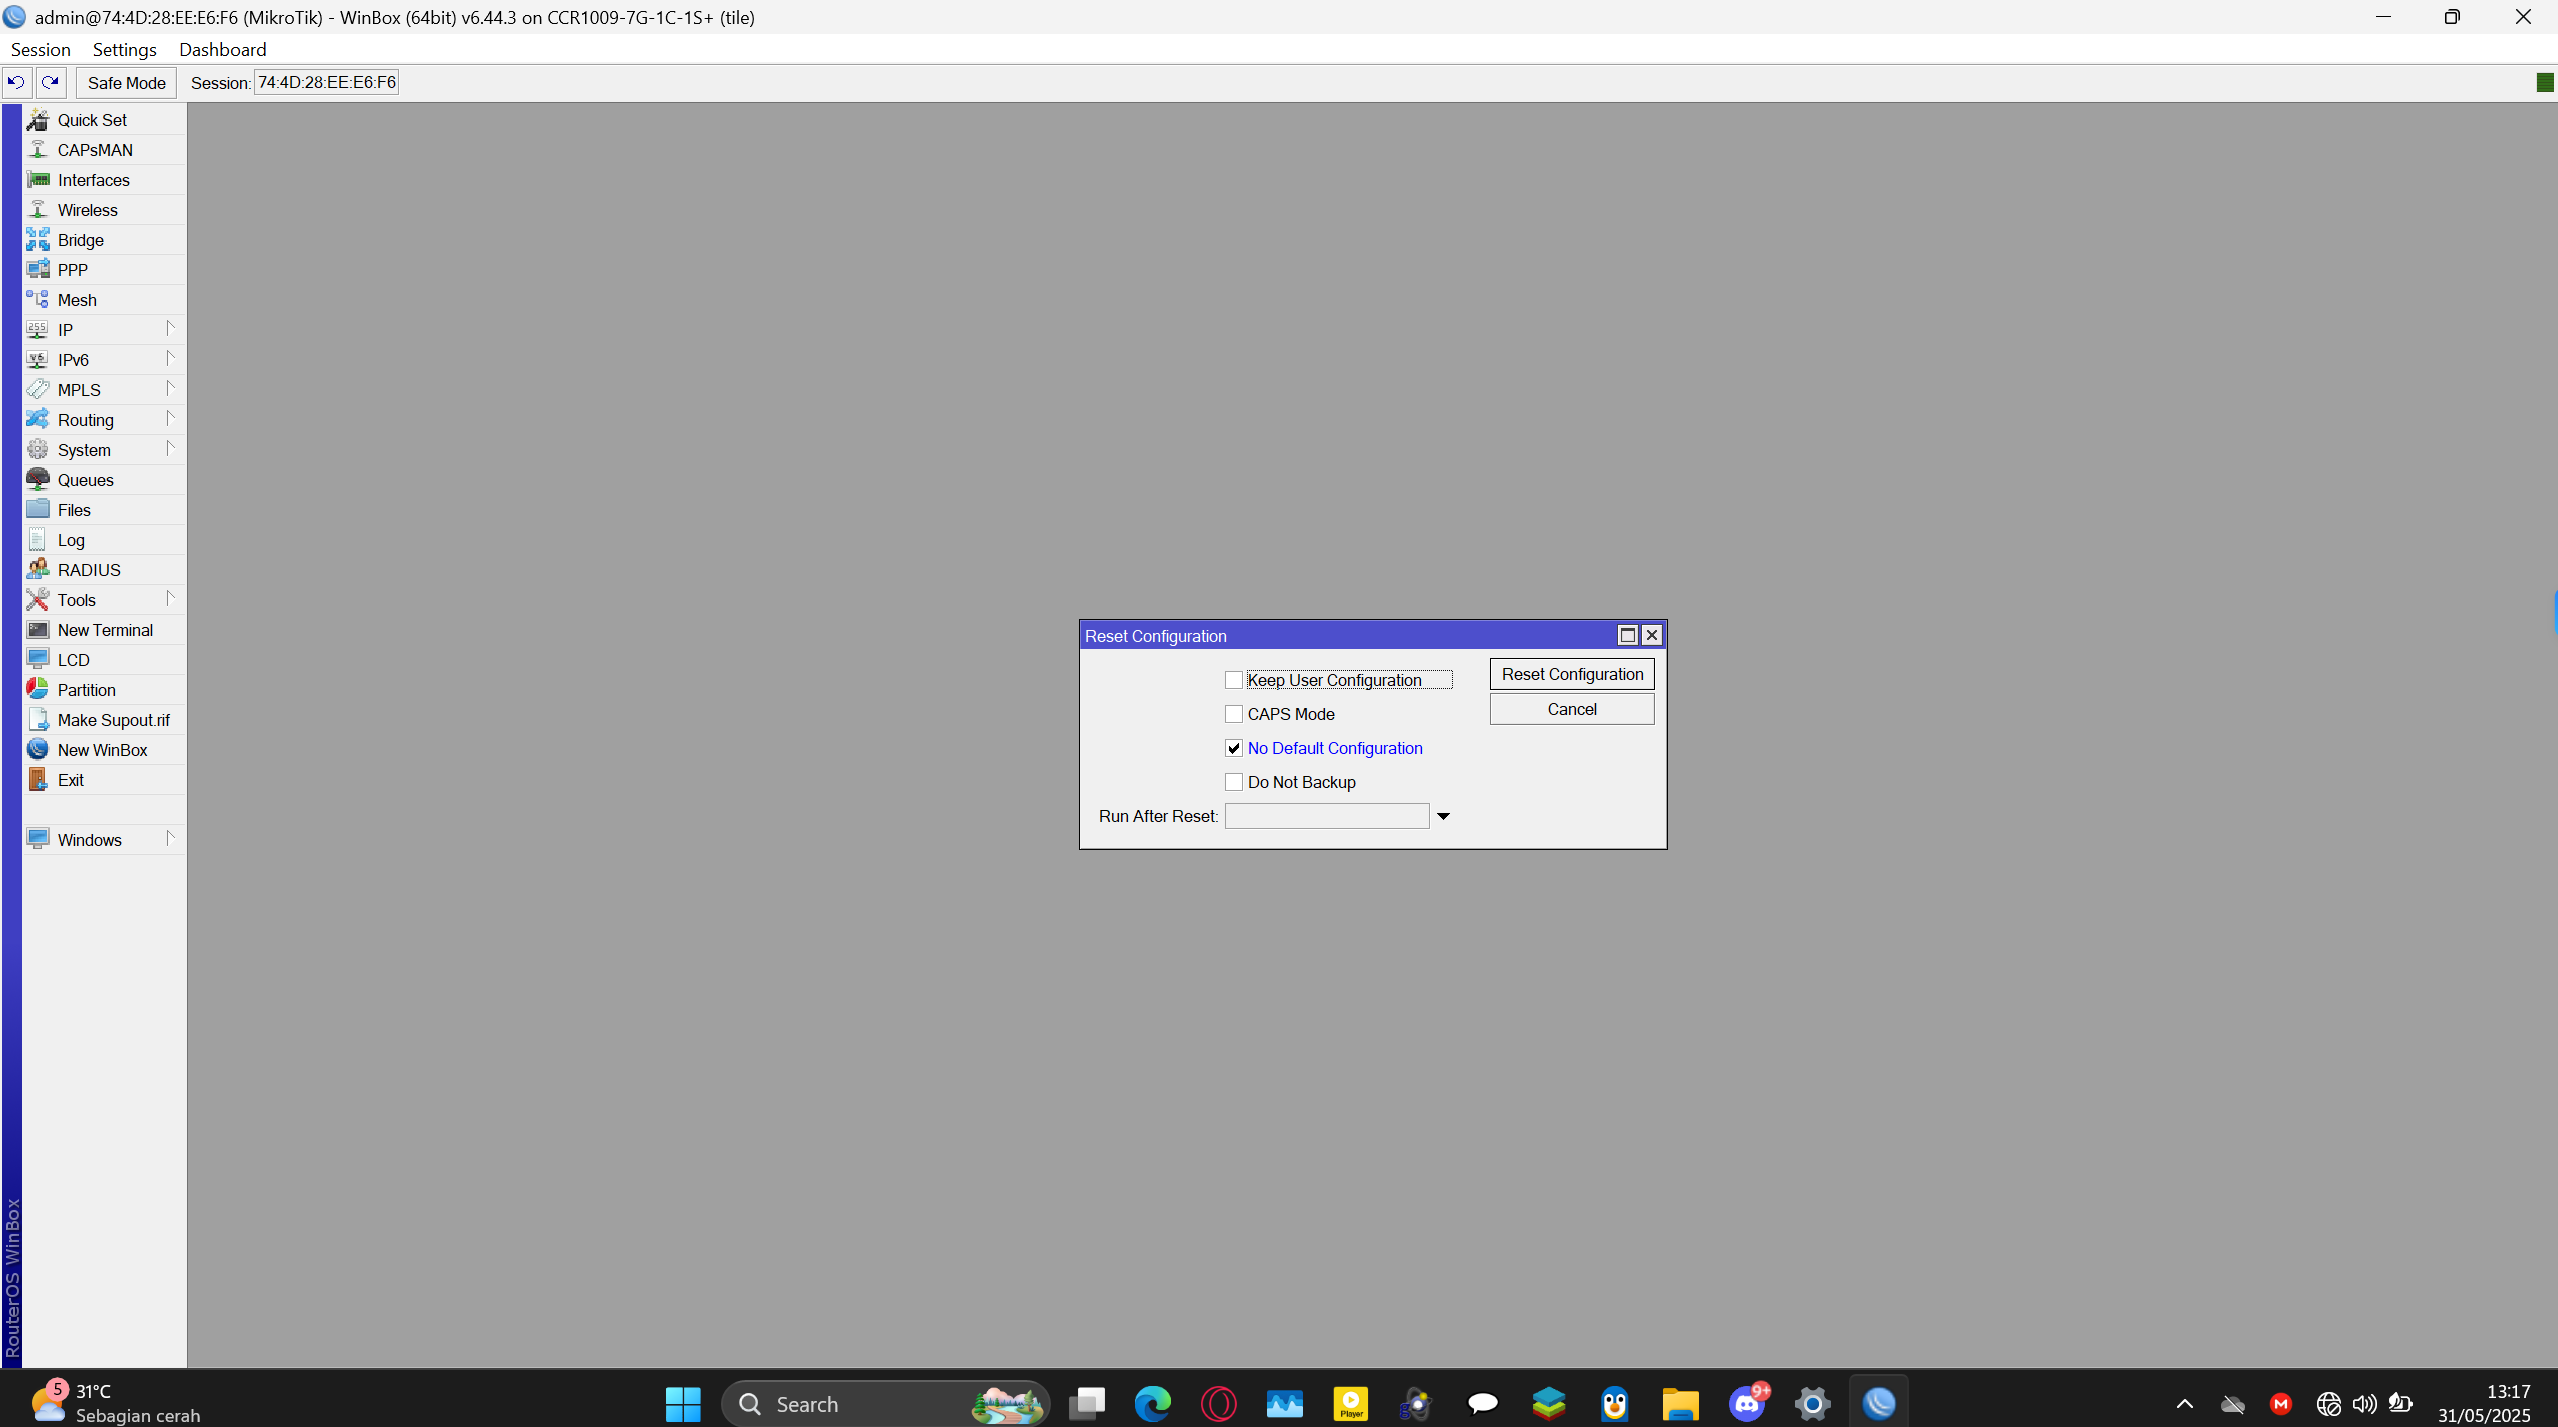
\includegraphics[width=0.5\linewidth]{P1/img/16.png}
        \caption{Reset Configuration}
        \label{fig:gambar4}
    \end{figure}
    \item Lakukan konfigurasi DCHP client pada router A terhadap ether 2
     \begin{figure}[H]
        \centering
        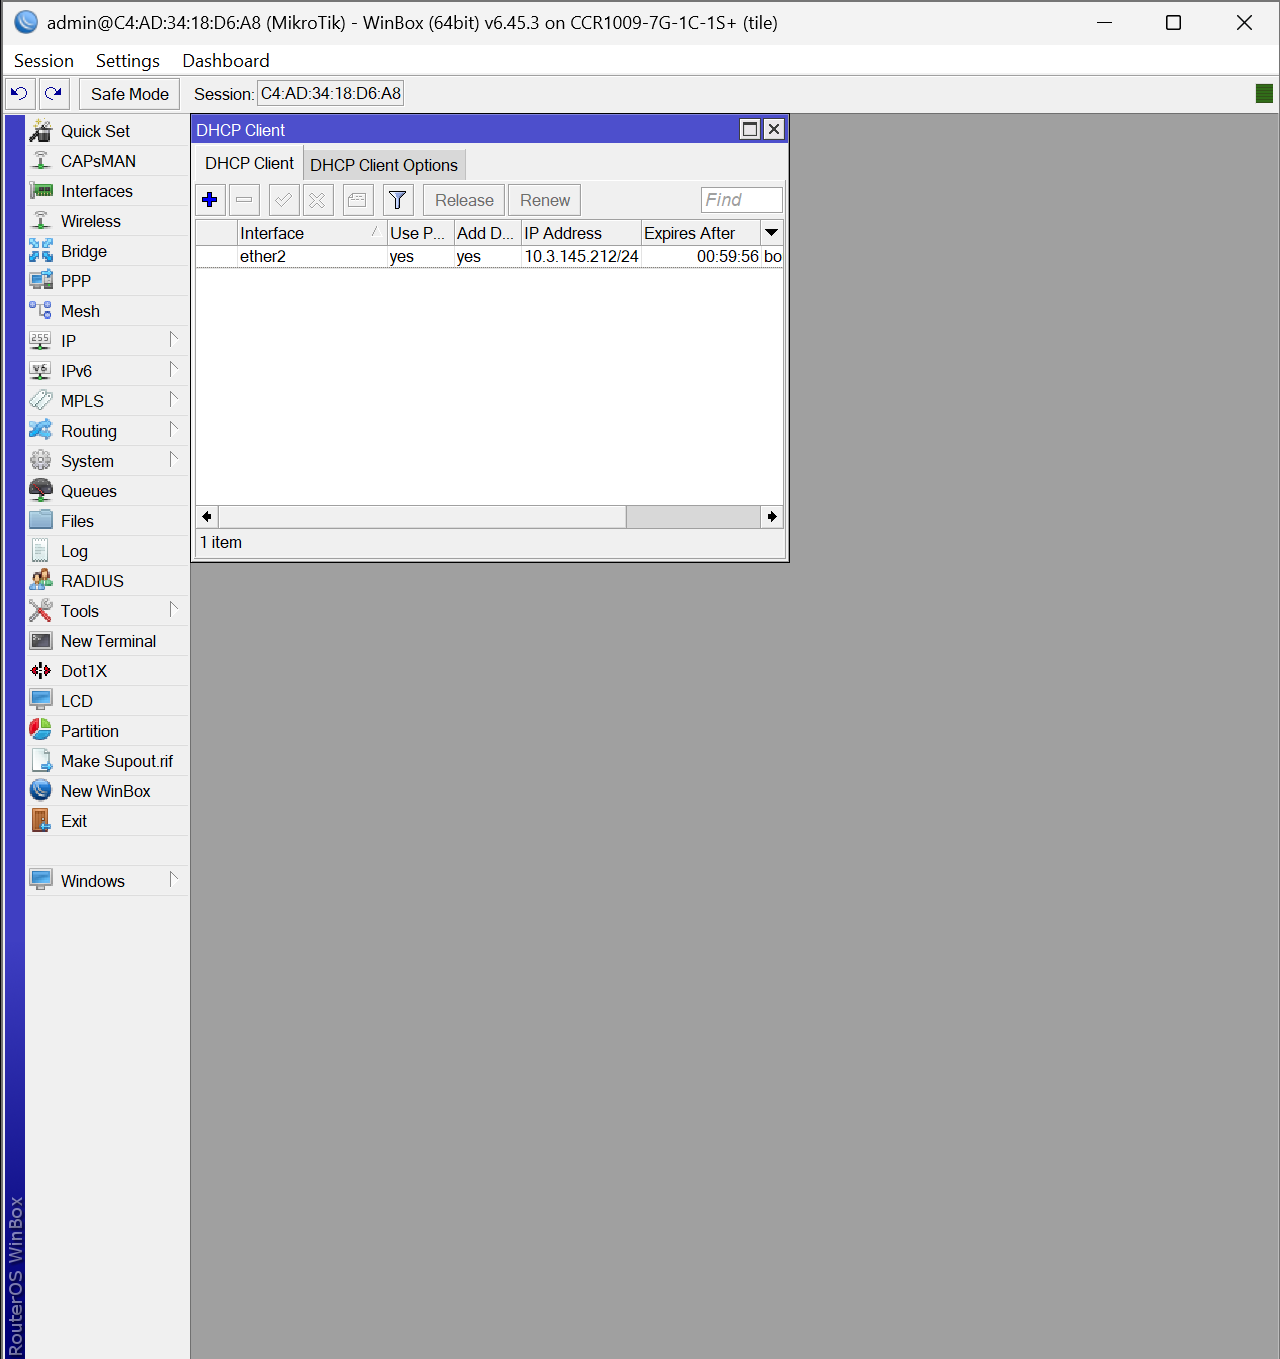
\includegraphics[width=0.5\linewidth]{P1/img/1.png}
        \caption{Atur DCHPnya}
        \label{fig:gambar4}
    \end{figure}
    \item Konfigurasi Firewall NAT seperti di gambar
     \begin{figure}[H]
        \centering
        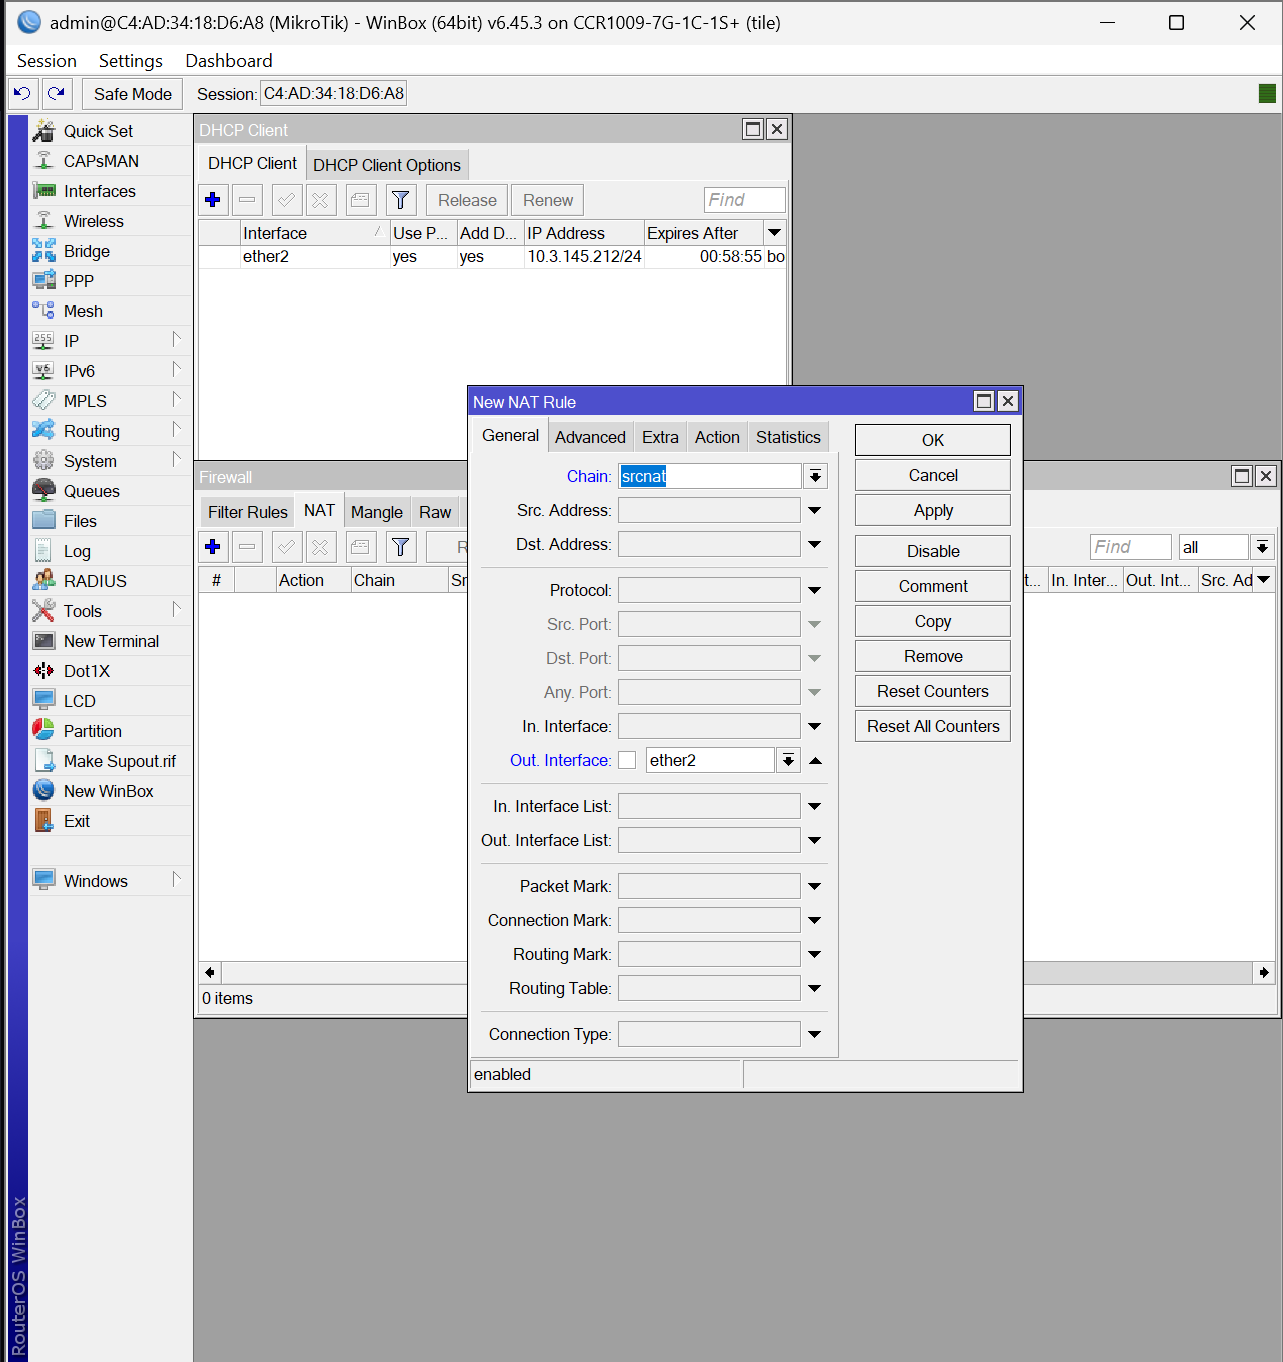
\includegraphics[width=0.5\linewidth]{P1/img/2.png}
        \caption{Konfigurasikan}
        \label{fig:gambar4}
    \end{figure}
       \begin{figure}[H]
        \centering
        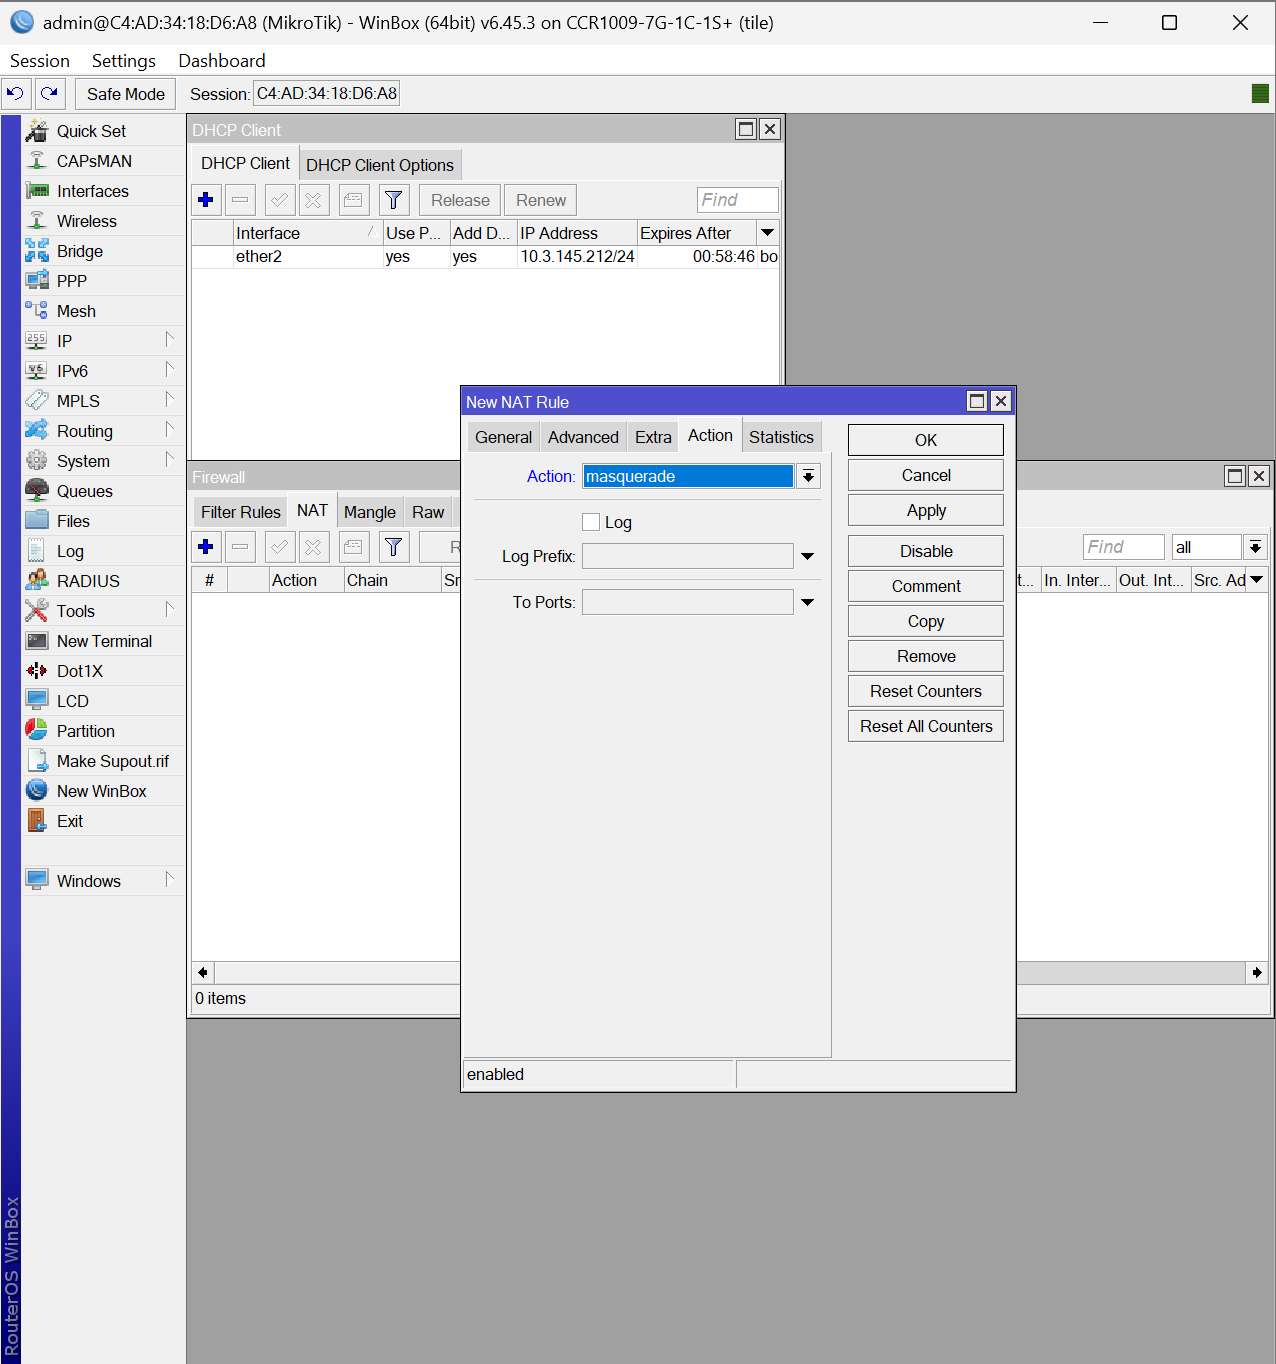
\includegraphics[width=0.5\linewidth]{P1/img/3.png}
        \caption{Konfigurasikan}
        \label{fig:gambar4}
    \end{figure}
    \item Sekarang konfigurasikan alamat IP lokalnya
     \begin{figure}[H]
        \centering
        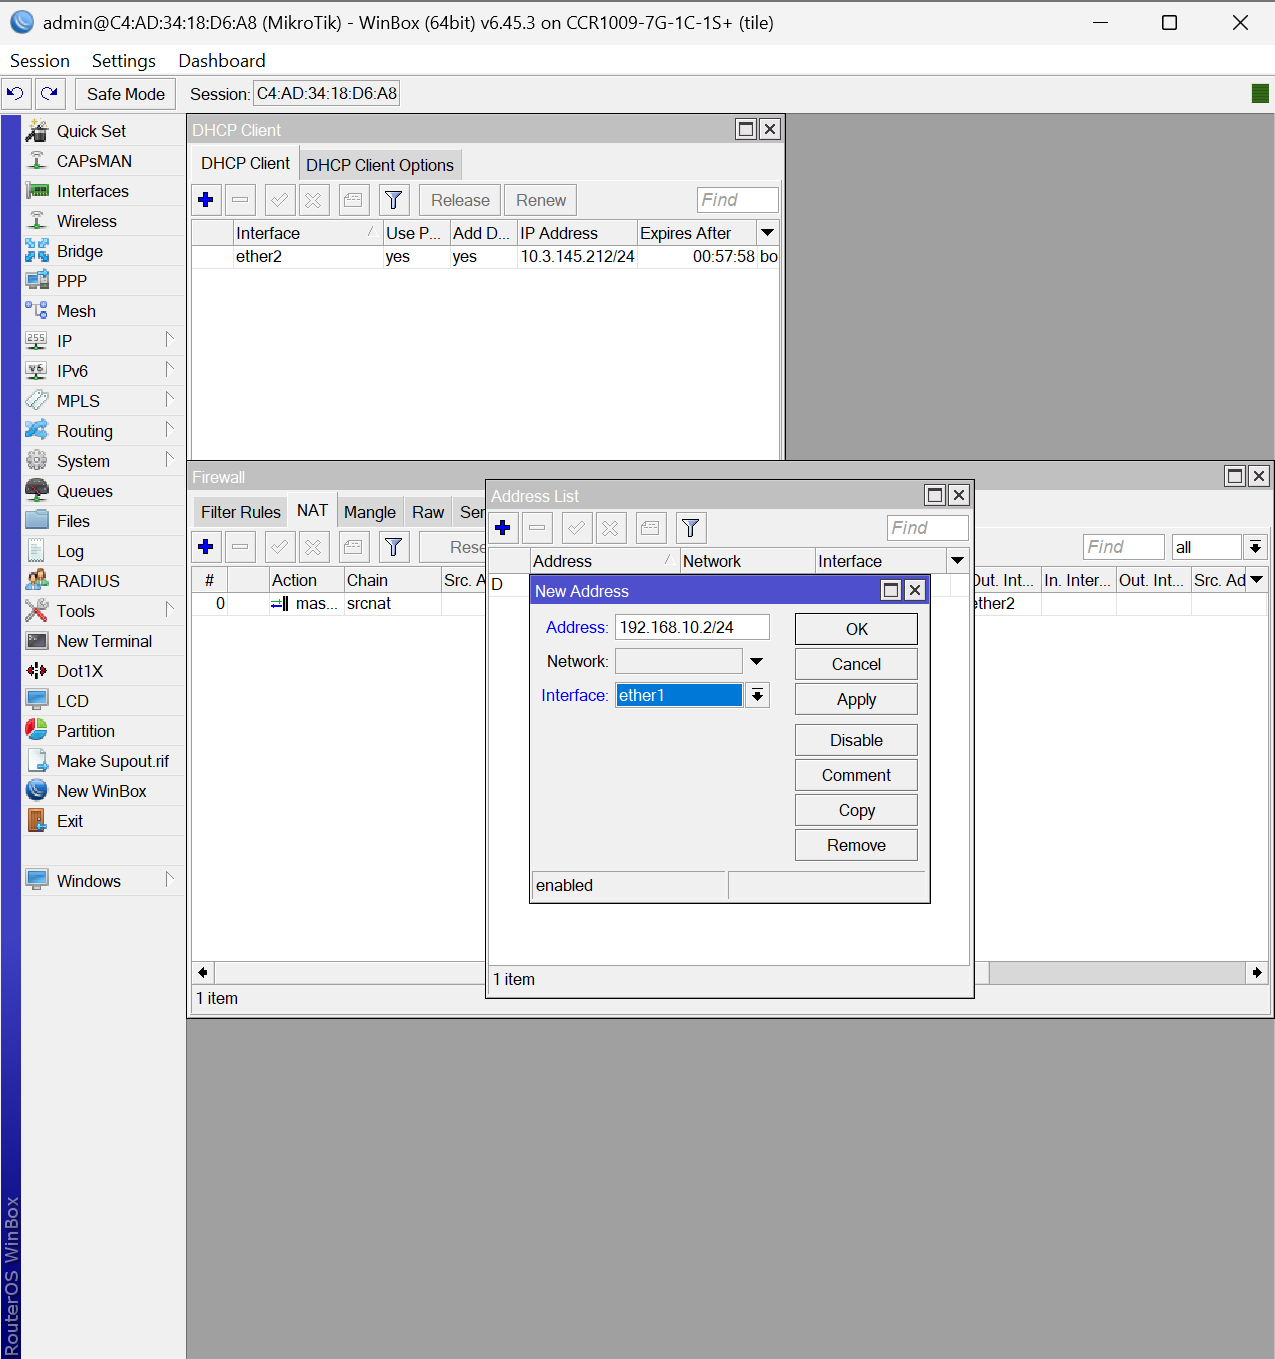
\includegraphics[width=0.5\linewidth]{P1/img/4.png}
        \caption{Konfigurasi alamat lokal}
        \label{fig:gambar4}
    \end{figure}
    \item konfigurasikan DHCP sever ke klien
     \begin{figure}[H]
        \centering
        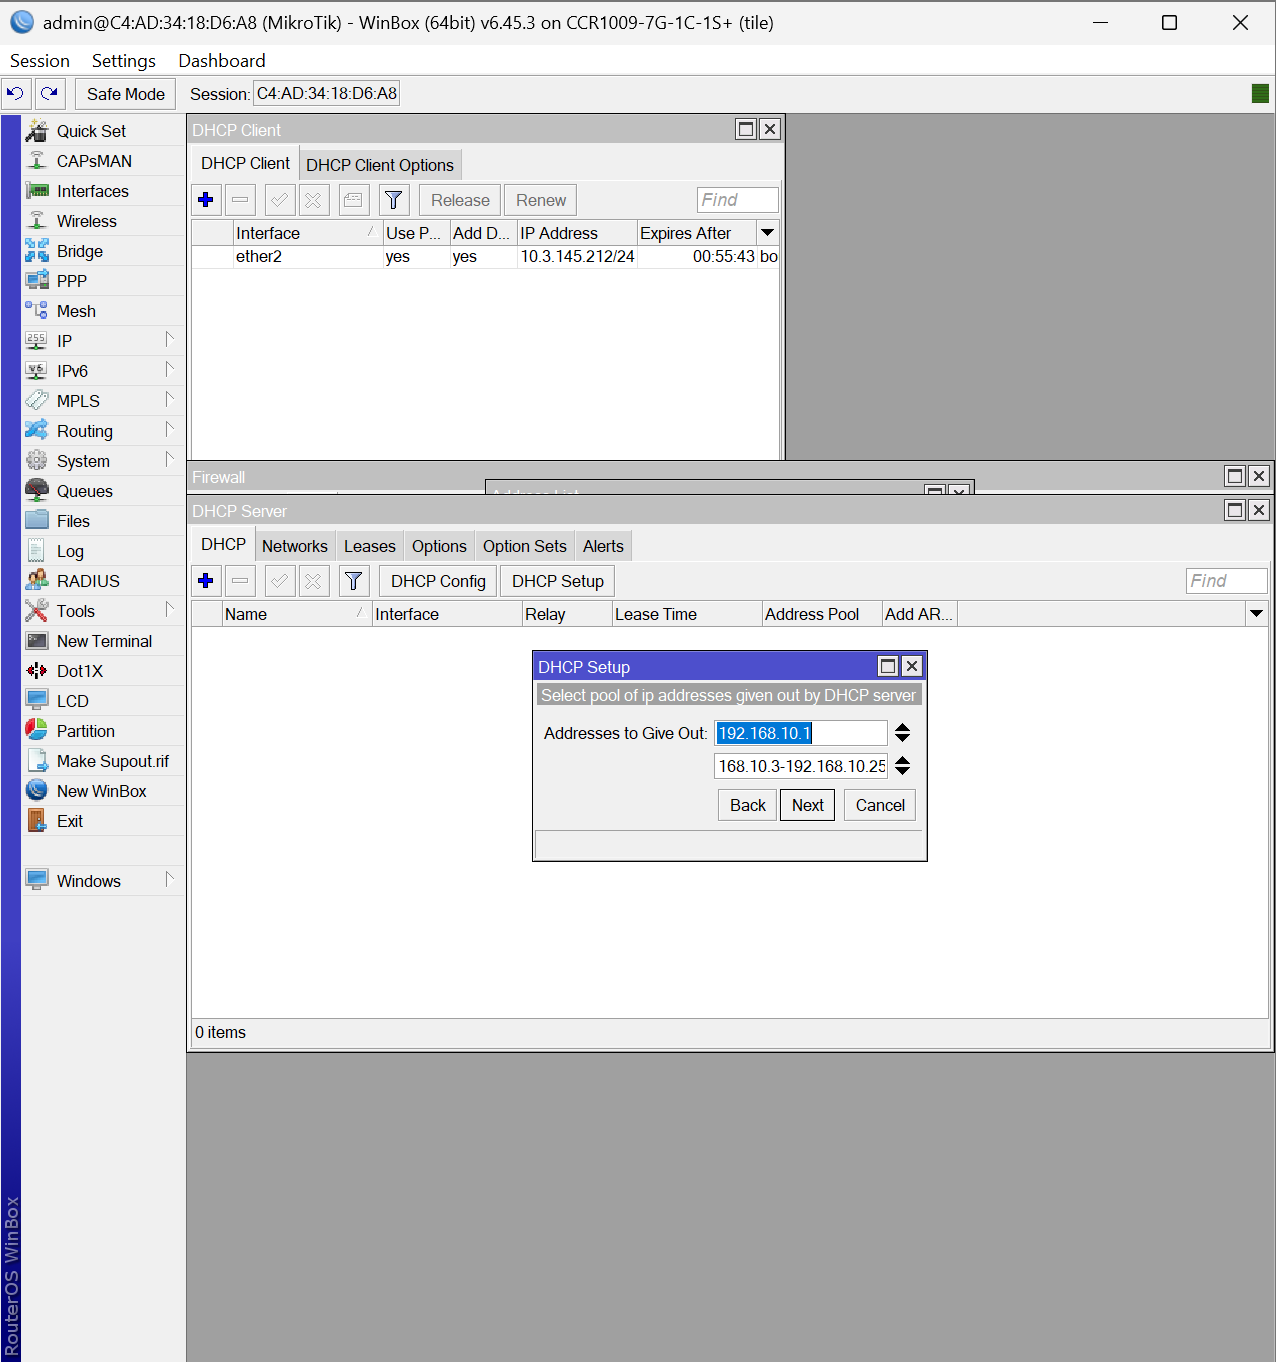
\includegraphics[width=0.5\linewidth]{P1/img/5.png}
        \caption{Atur DCHP servernya}
        \label{fig:gambar4}
    \end{figure}
    \item Aktifkan Proxy ARP
     \begin{figure}[H]
        \centering
        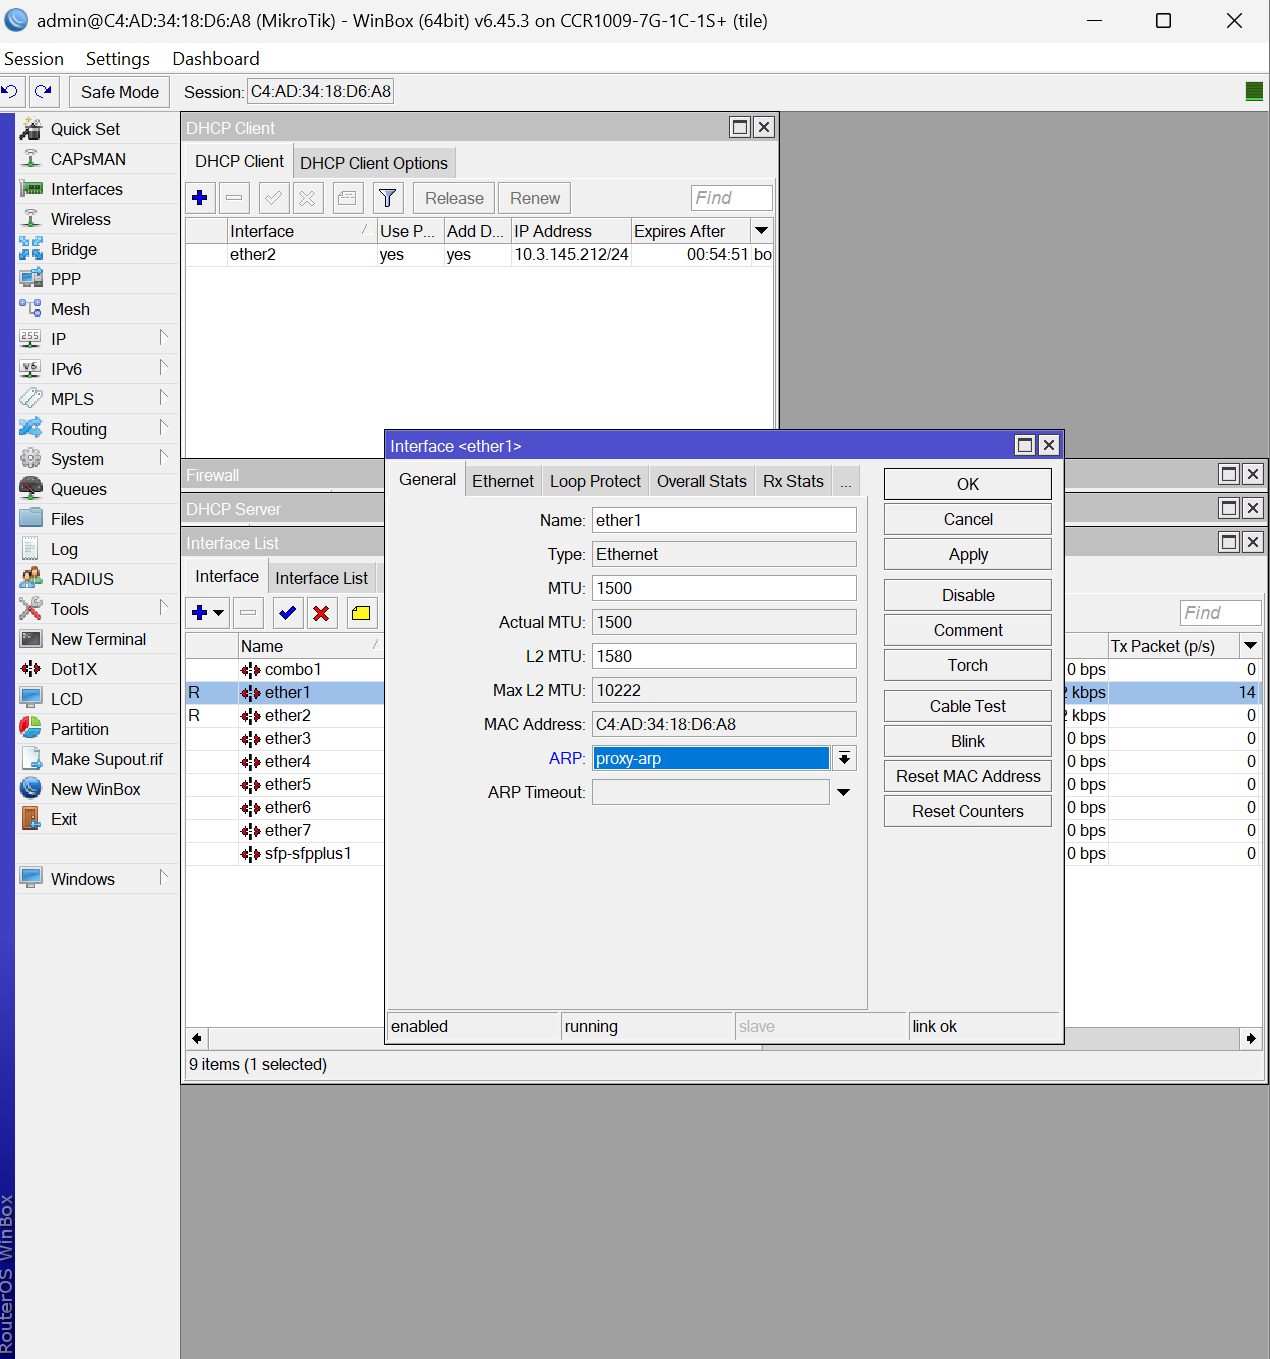
\includegraphics[width=0.5\linewidth]{P1/img/6.png}
        \caption{Proxy ARP}
        \label{fig:gambar4}
    \end{figure}
    \item Konfigurasi PPTP server VPN
     \begin{figure}[H]
        \centering
        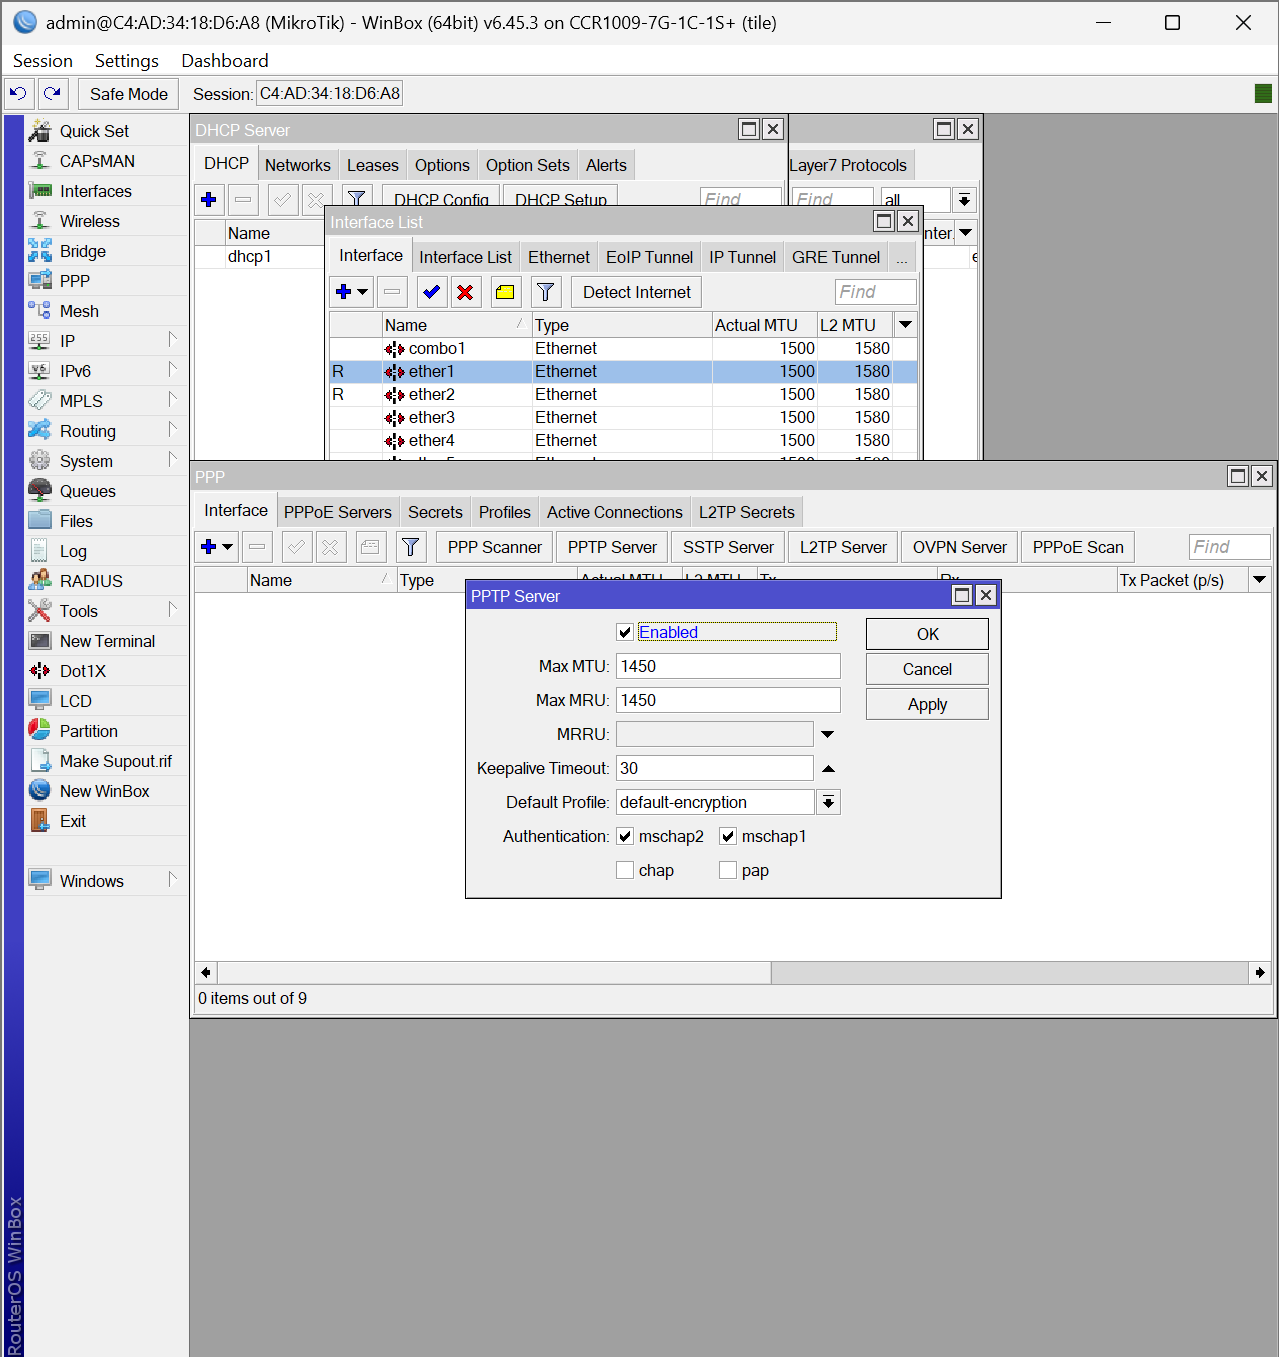
\includegraphics[width=0.5\linewidth]{P1/img/7.png}
        \caption{VPN server}
        \label{fig:gambar4}
    \end{figure}
     \begin{figure}[H]
        \centering
        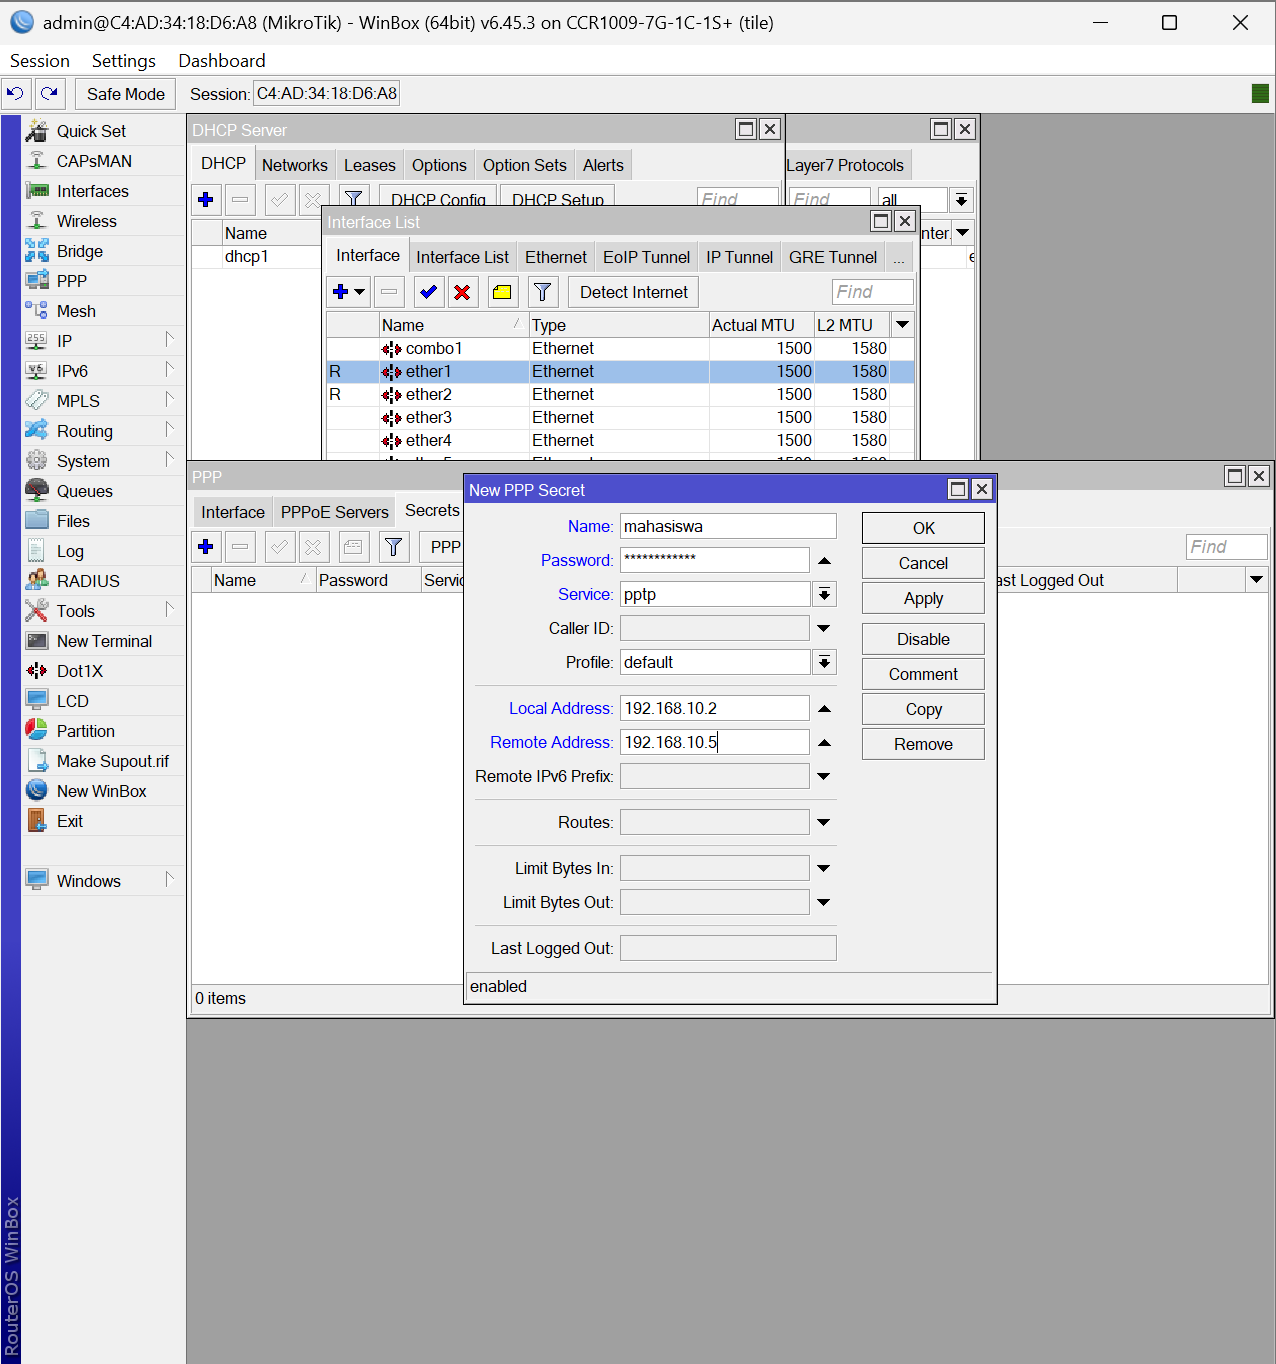
\includegraphics[width=0.5\linewidth]{P1/img/8.png}
        \caption{buat user dan passwordnya}
        \label{fig:gambar4}
    \end{figure}
    \item konfigurasikan PPTP clinet di laptop
     \begin{figure}[H]
        \centering
        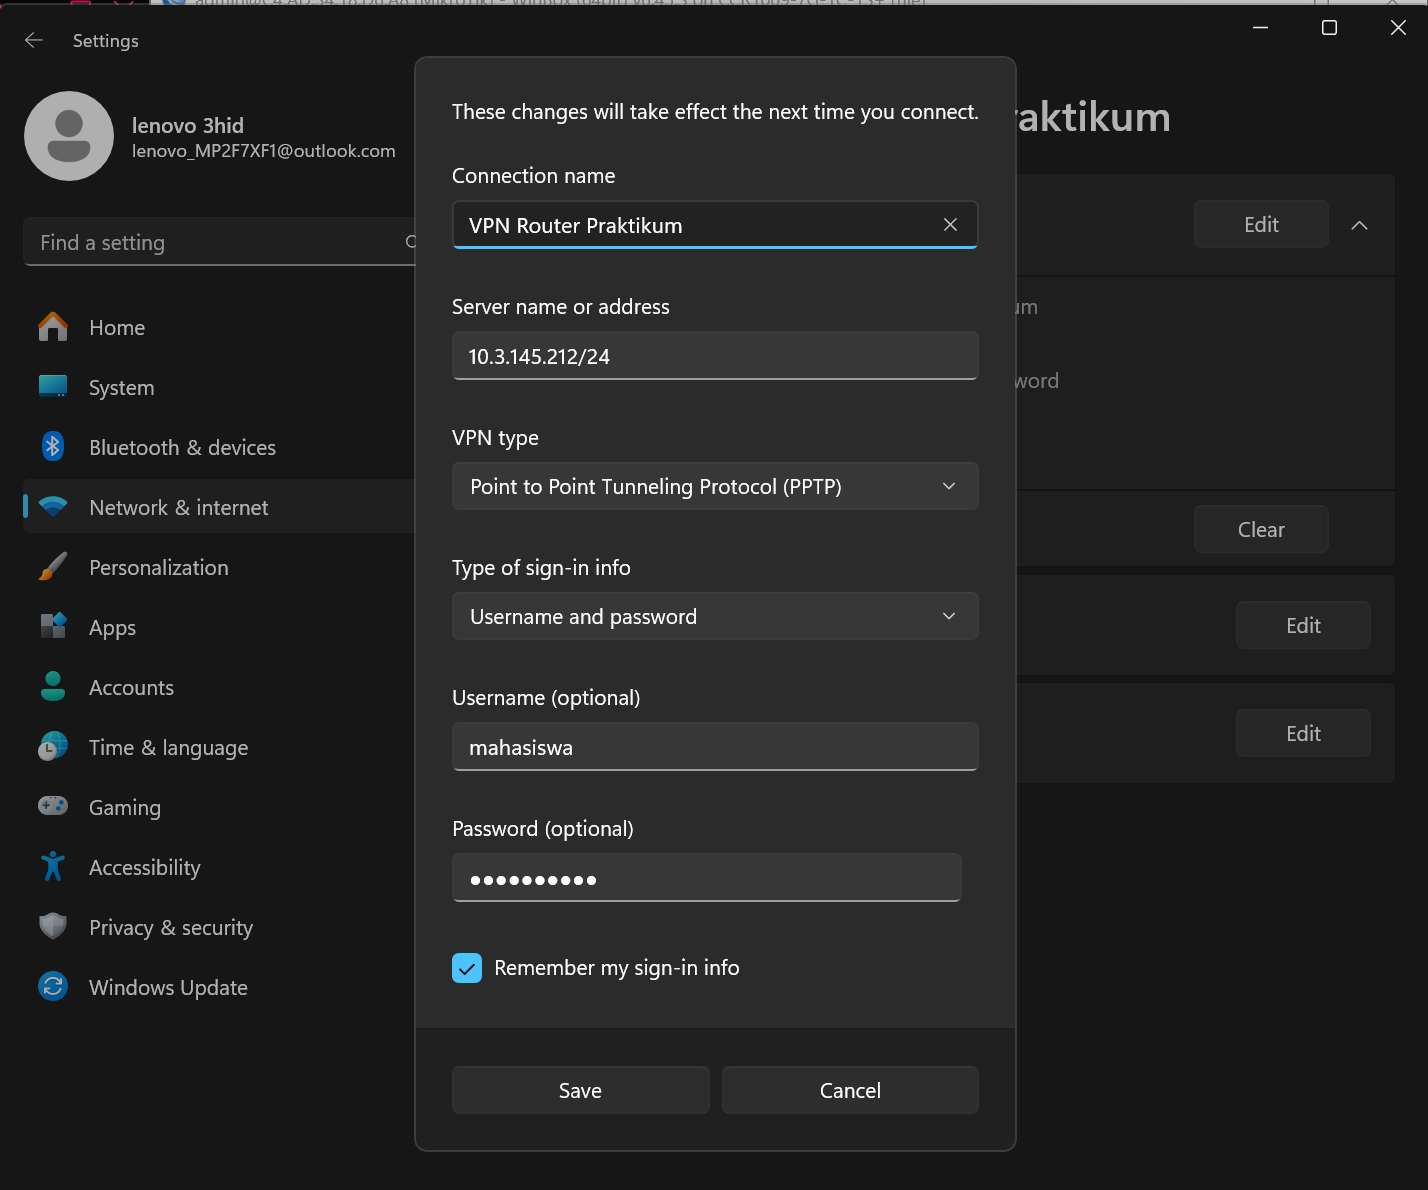
\includegraphics[width=0.5\linewidth]{P1/img/9.png}
        \caption{Buatkan konfigurasi}
        \label{fig:gambar4}
    \end{figure}
    \item Uji Coba Konfigurasinya
     \begin{figure}[H]
        \centering
        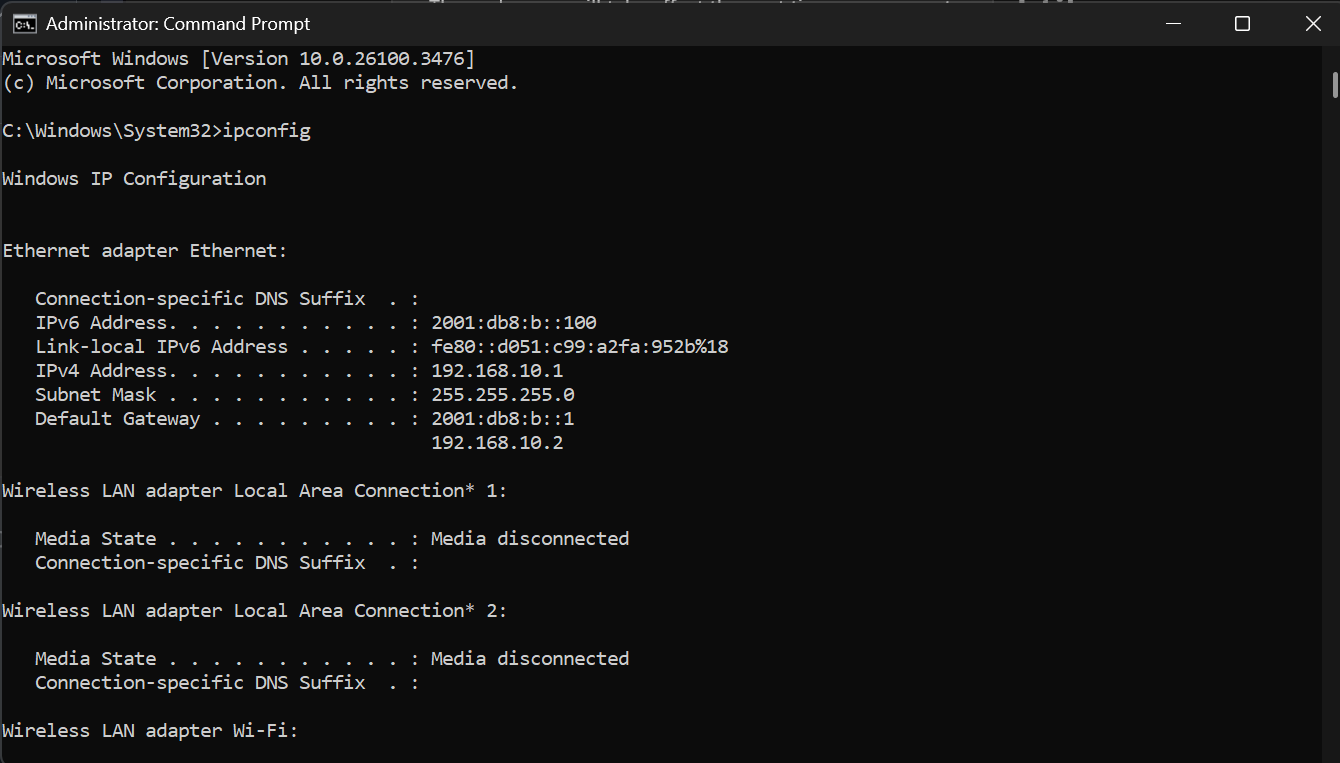
\includegraphics[width=0.5\linewidth]{P1/img/10.png}
        \caption{Uji ping}
        \label{fig:gambar4}
    \end{figure}
\begin{figure}[H]
        \centering
        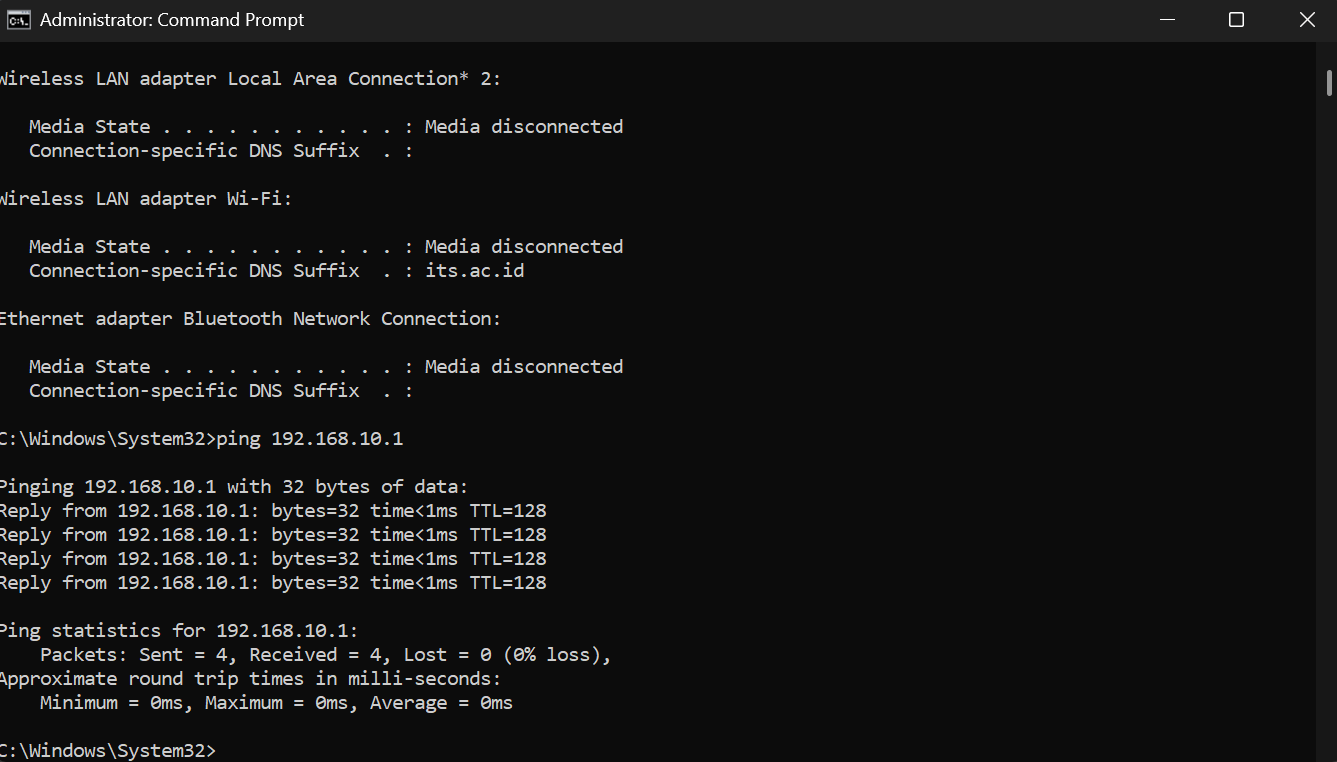
\includegraphics[width=0.5\linewidth]{P1/img/11.png}
        \caption{Uji ping}
        \label{fig:gambar4}
    \end{figure}
\end{enumerate}

\subsection{Konfigurasi QOS PC dengan Router (Router Tidak perlu di Reset)}
\begin{enumerate}
    \item Buat aturan Simple Queue untuk membatasi kecepatan upload
    \begin{figure}[H]
        \centering
        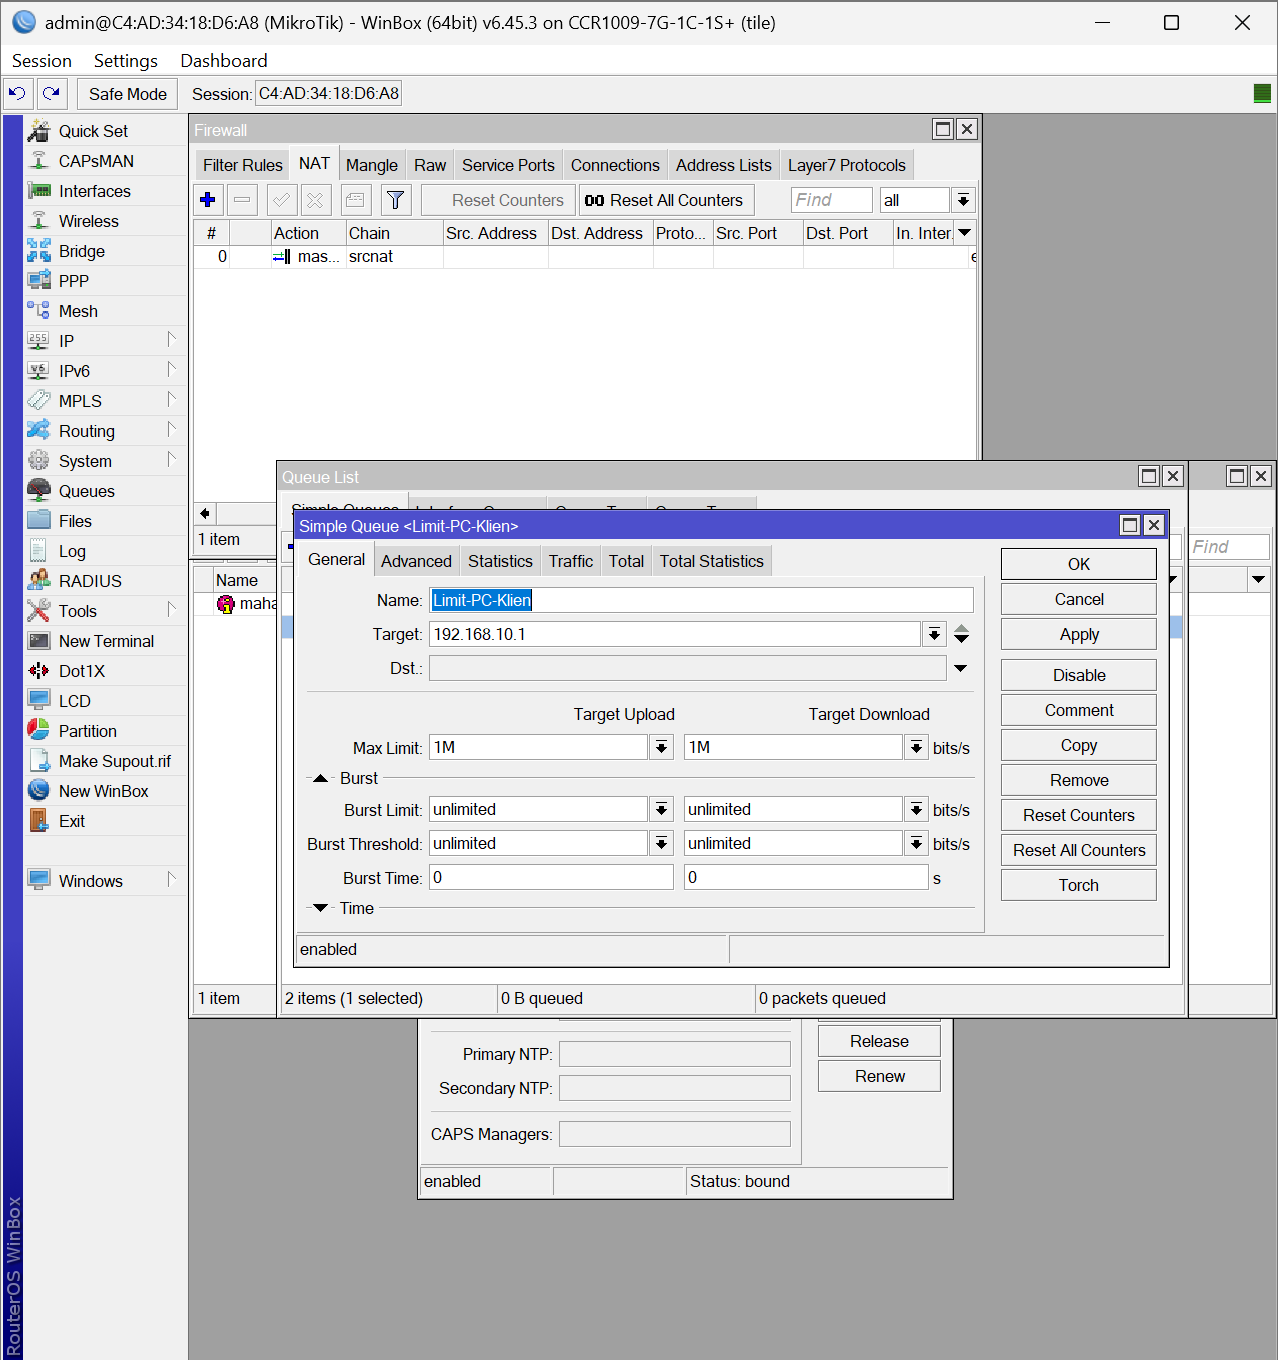
\includegraphics[width=0.5\linewidth]{P1/img/12.png}
        \caption{Aturan Queue nya}
        \label{fig:gambar4}
    \end{figure}
    \item Pantau penggunaan traffic
    \begin{figure}[H]
        \centering
        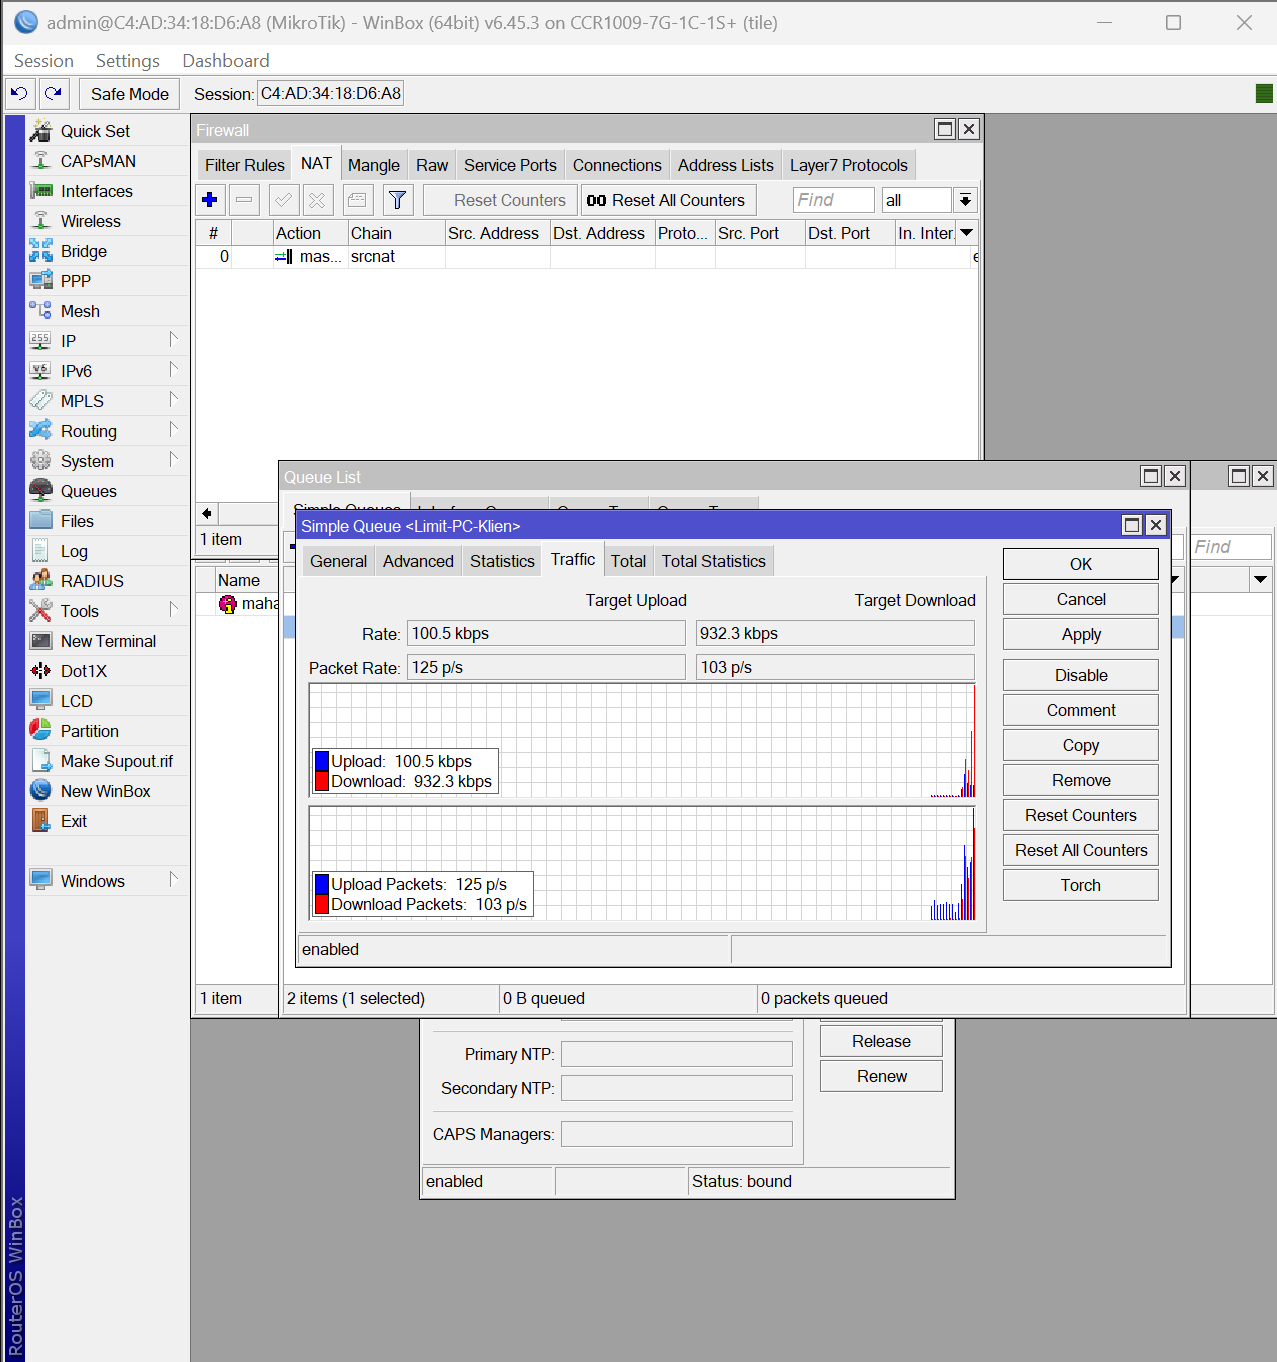
\includegraphics[width=0.5\linewidth]{P1/img/13.png}
        \caption{Uji ping}
        \label{fig:gambar4}
    \end{figure}
    \item Uji saat queue aktif dan tidak akrif
    \begin{figure}[H]
        \centering
        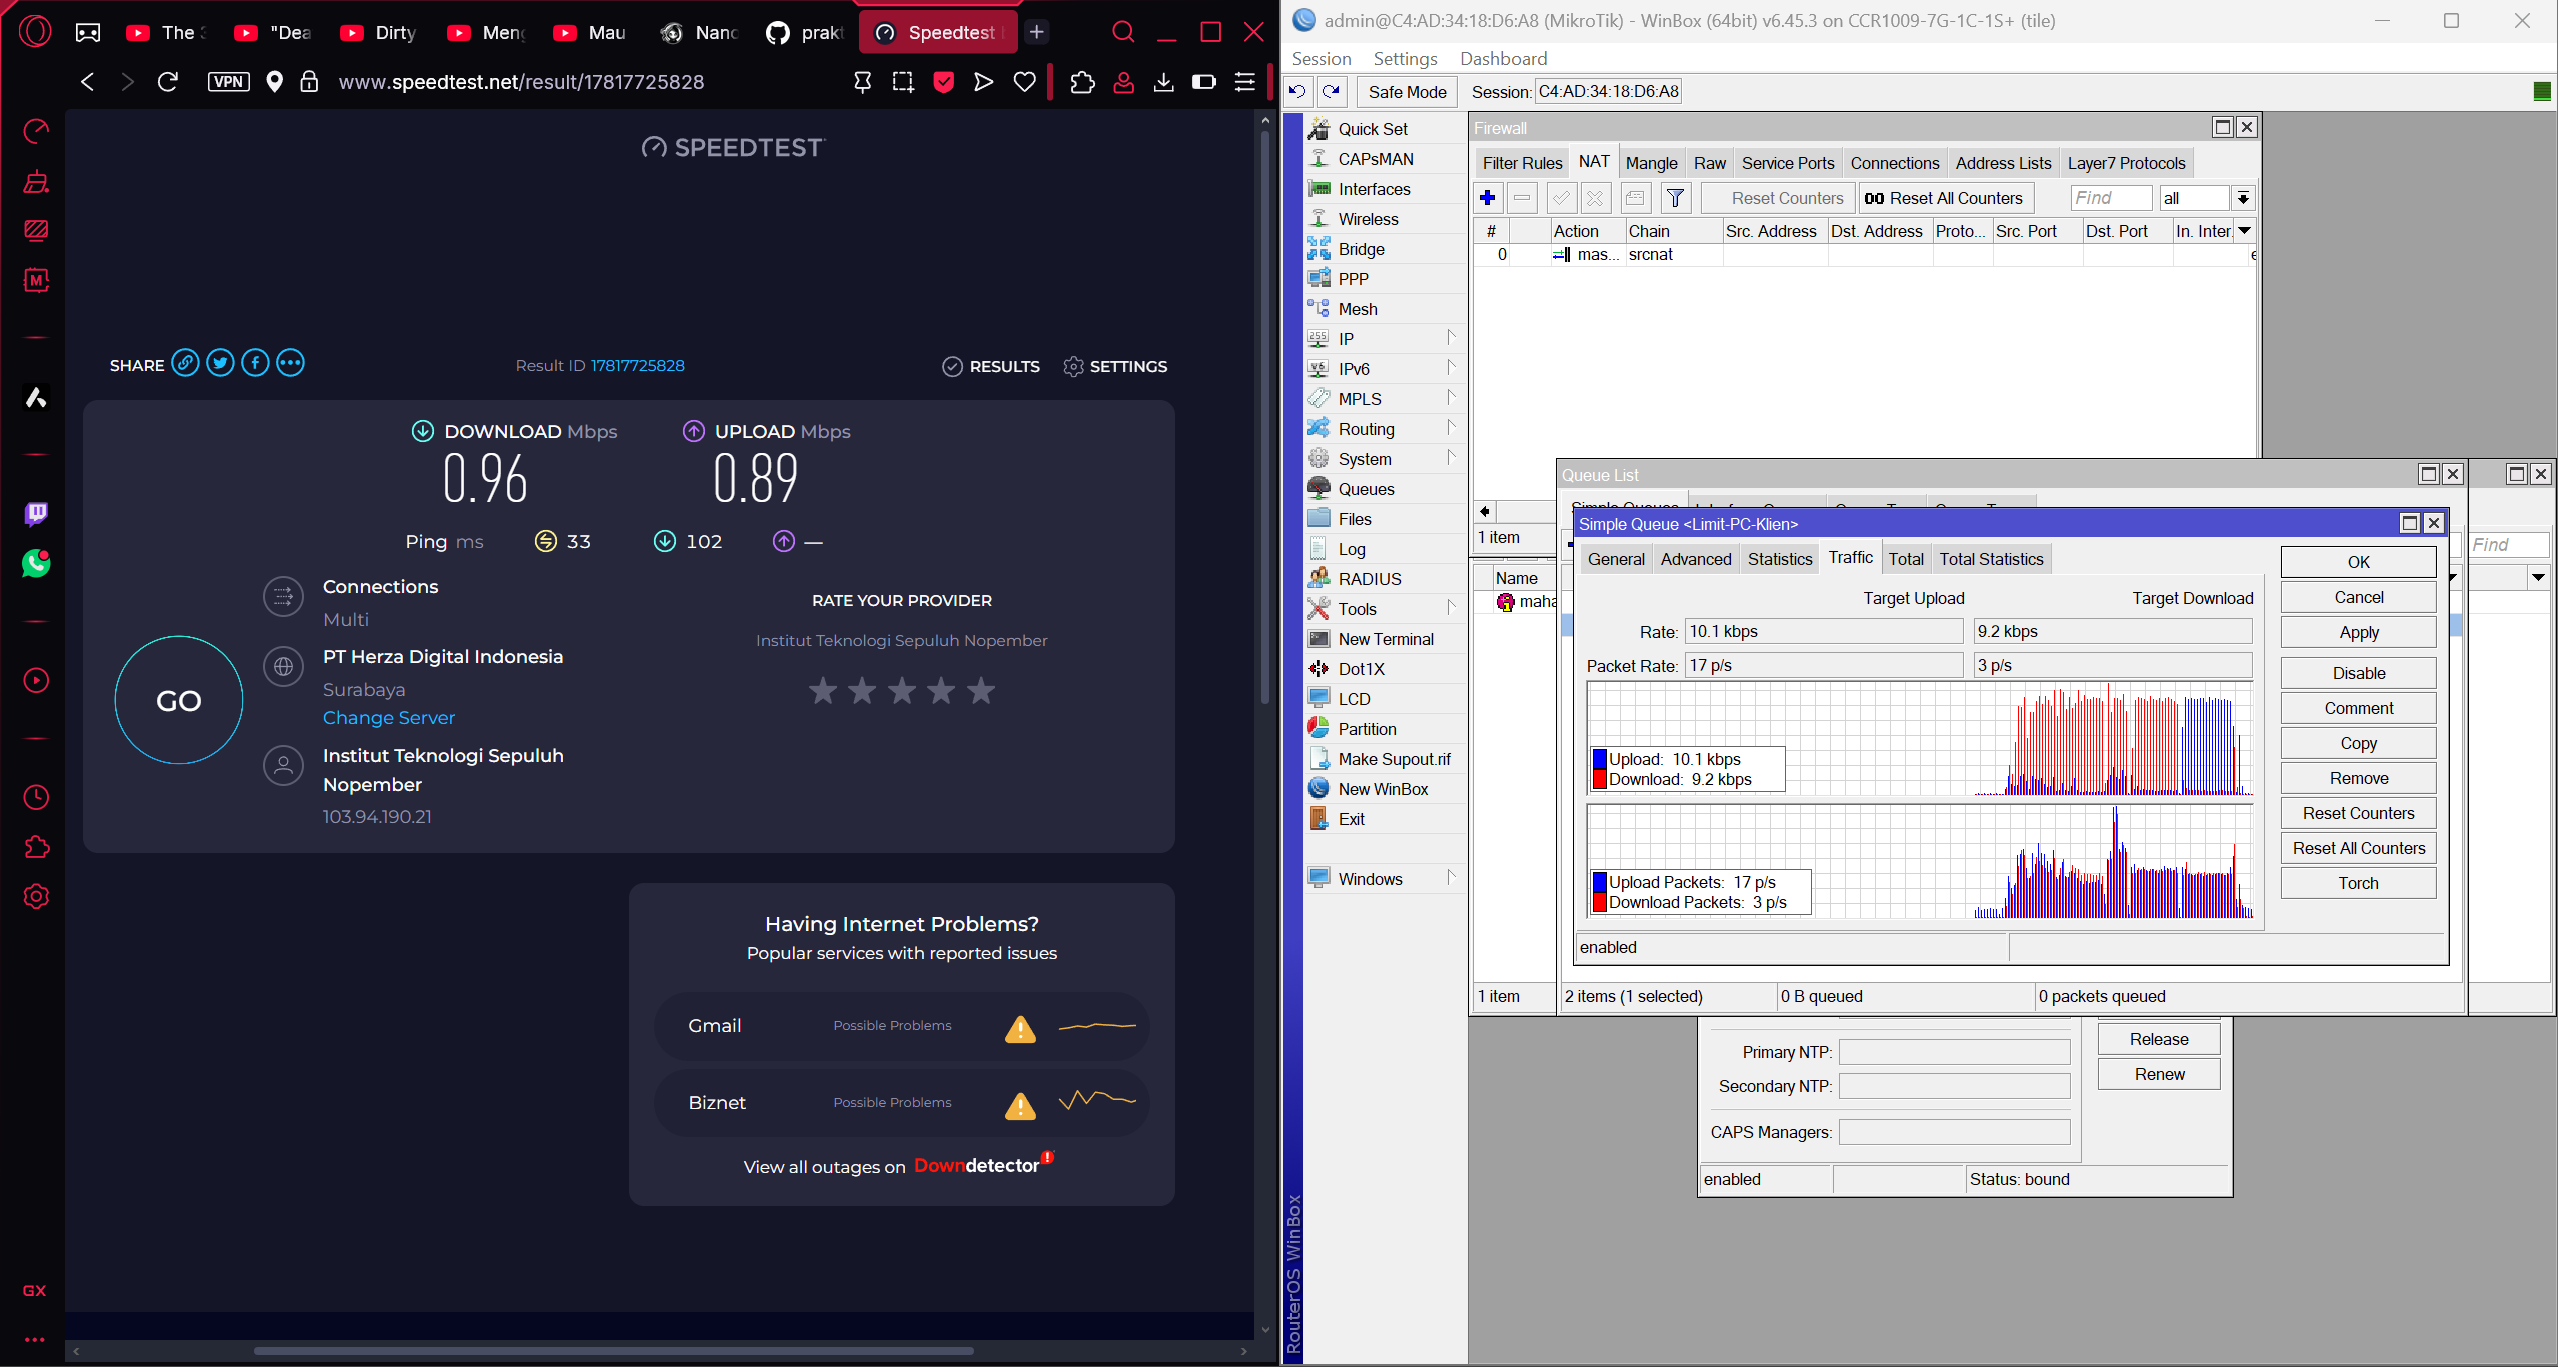
\includegraphics[width=0.5\linewidth]{P1/img/14.png}
        \caption{Saat queue di aktifkan}
        \label{fig:gambar4}
    \end{figure}
    \begin{figure}[H]
        \centering
        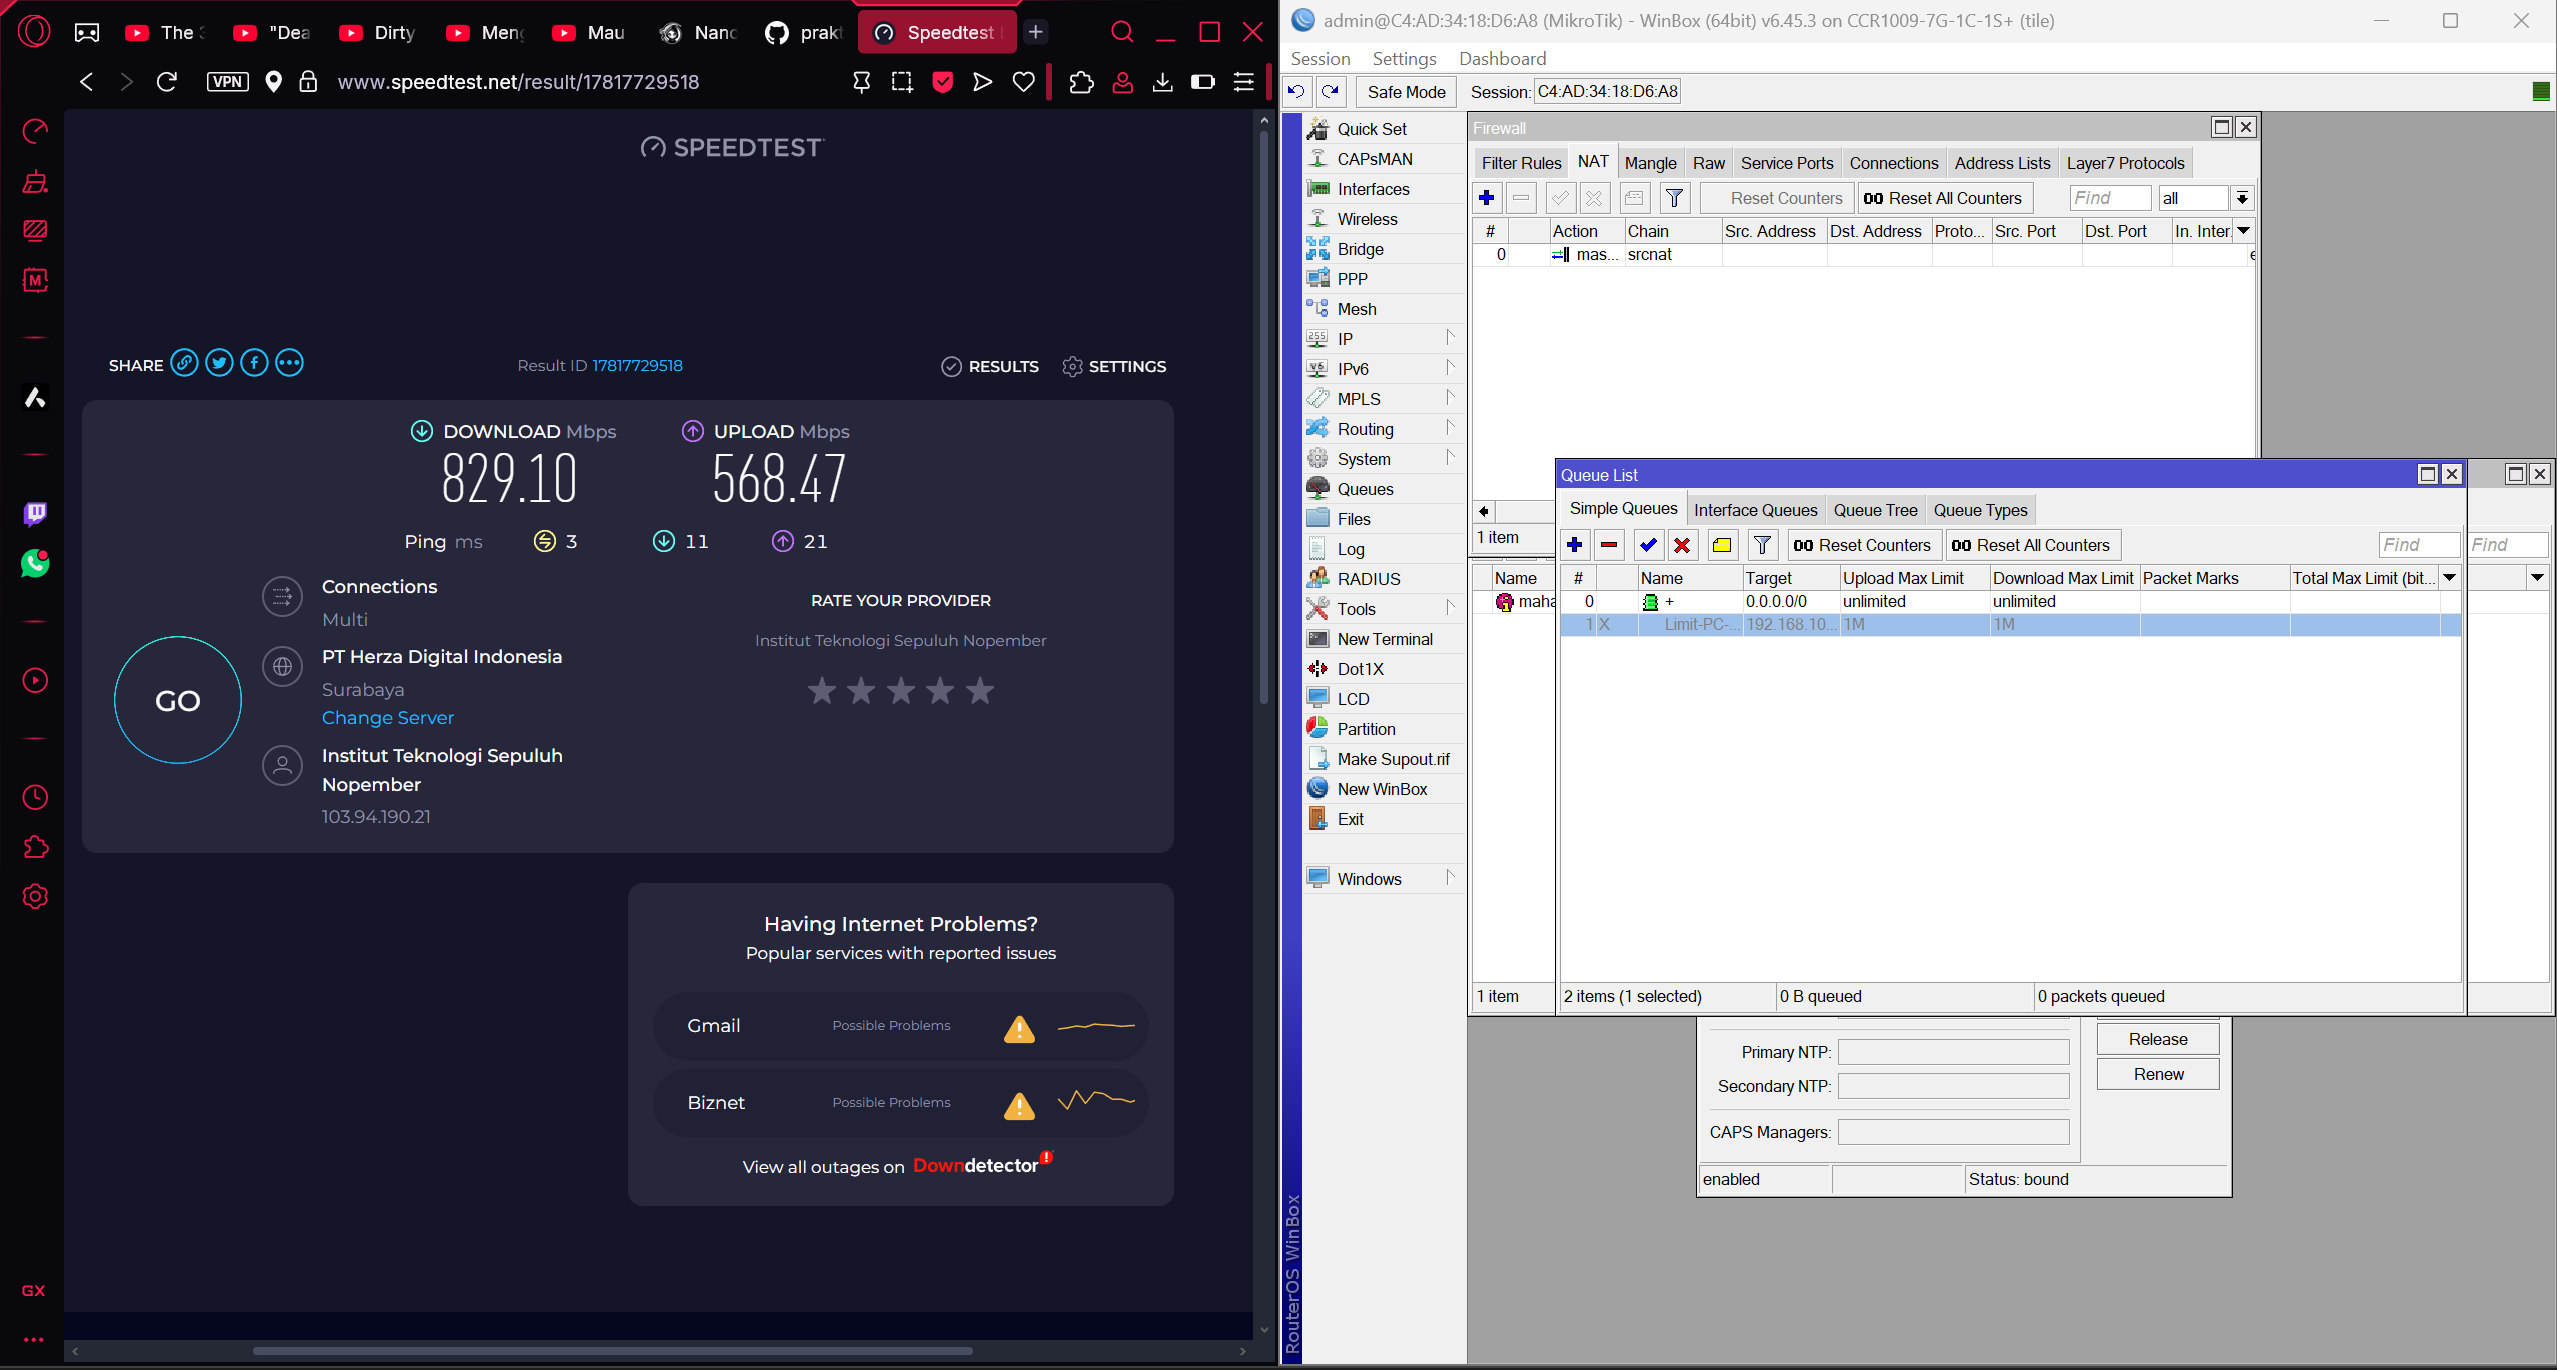
\includegraphics[width=0.5\linewidth]{P1/img/15.png}
        \caption{Saat queue tidak aktif}
        \label{fig:gambar4}
    \end{figure}
\end{enumerate}

\section{Analisis Hasil Percobaan}
Pada praktikum ini dilakukan konfigurasi koneksi VPN berbasis PPTP (Point-to-Point Tunneling Protocol) menggunakan perangkat MikroTik. Praktikum bertujuan untuk memahami bagaimana membangun koneksi jaringan privat secara aman melalui internet menggunakan tunneling. Topologi yang digunakan terdiri dari dua buah router yang masing-masing terhubung dengan satu klien PC, dan dikonfigurasi untuk saling terhubung secara virtual melalui VPN. Router pertama dihubungkan ke internet menggunakan DHCP Client dan NAT, sedangkan router kedua dikonfigurasi untuk menerima koneksi VPN.

Langkah pertama adalah mereset konfigurasi router untuk memastikan tidak ada konflik pengaturan. Router pertama disambungkan ke internet melalui interface tertentu (misalnya ether3), dikonfigurasi sebagai DHCP client, lalu ditambahkan IP lokal pada ether1. DHCP server juga diaktifkan untuk mendistribusikan IP ke klien yang terhubung ke ether1. Selanjutnya, aturan NAT bertipe \texttt{masquerade} dibuat untuk memungkinkan akses internet bagi jaringan lokal. Kemudian dilakukan konfigurasi VPN PPTP pada router, mulai dari mengaktifkan server PPTP, membuat user VPN, hingga menetapkan IP lokal dan remote untuk koneksi tunnel. Klien VPN di laptop lalu dikonfigurasi dan berhasil terhubung menggunakan kredensial yang telah dibuat.

Pengujian dilakukan dengan perintah \texttt{ping} dari PC klien VPN menuju IP lokal router dan IP PC lain di jaringan internal. Hasil pengujian menunjukkan koneksi berhasil dilakukan tanpa packet loss, membuktikan bahwa tunnel PPTP berfungsi sebagaimana mestinya. Dengan demikian, koneksi antar dua jaringan yang terpisah secara fisik dapat dijembatani melalui internet menggunakan VPN PPTP yang aman dan terenkripsi.


\section{Hasil Tugas Modul}

\begin{figure}[H]
        \centering
        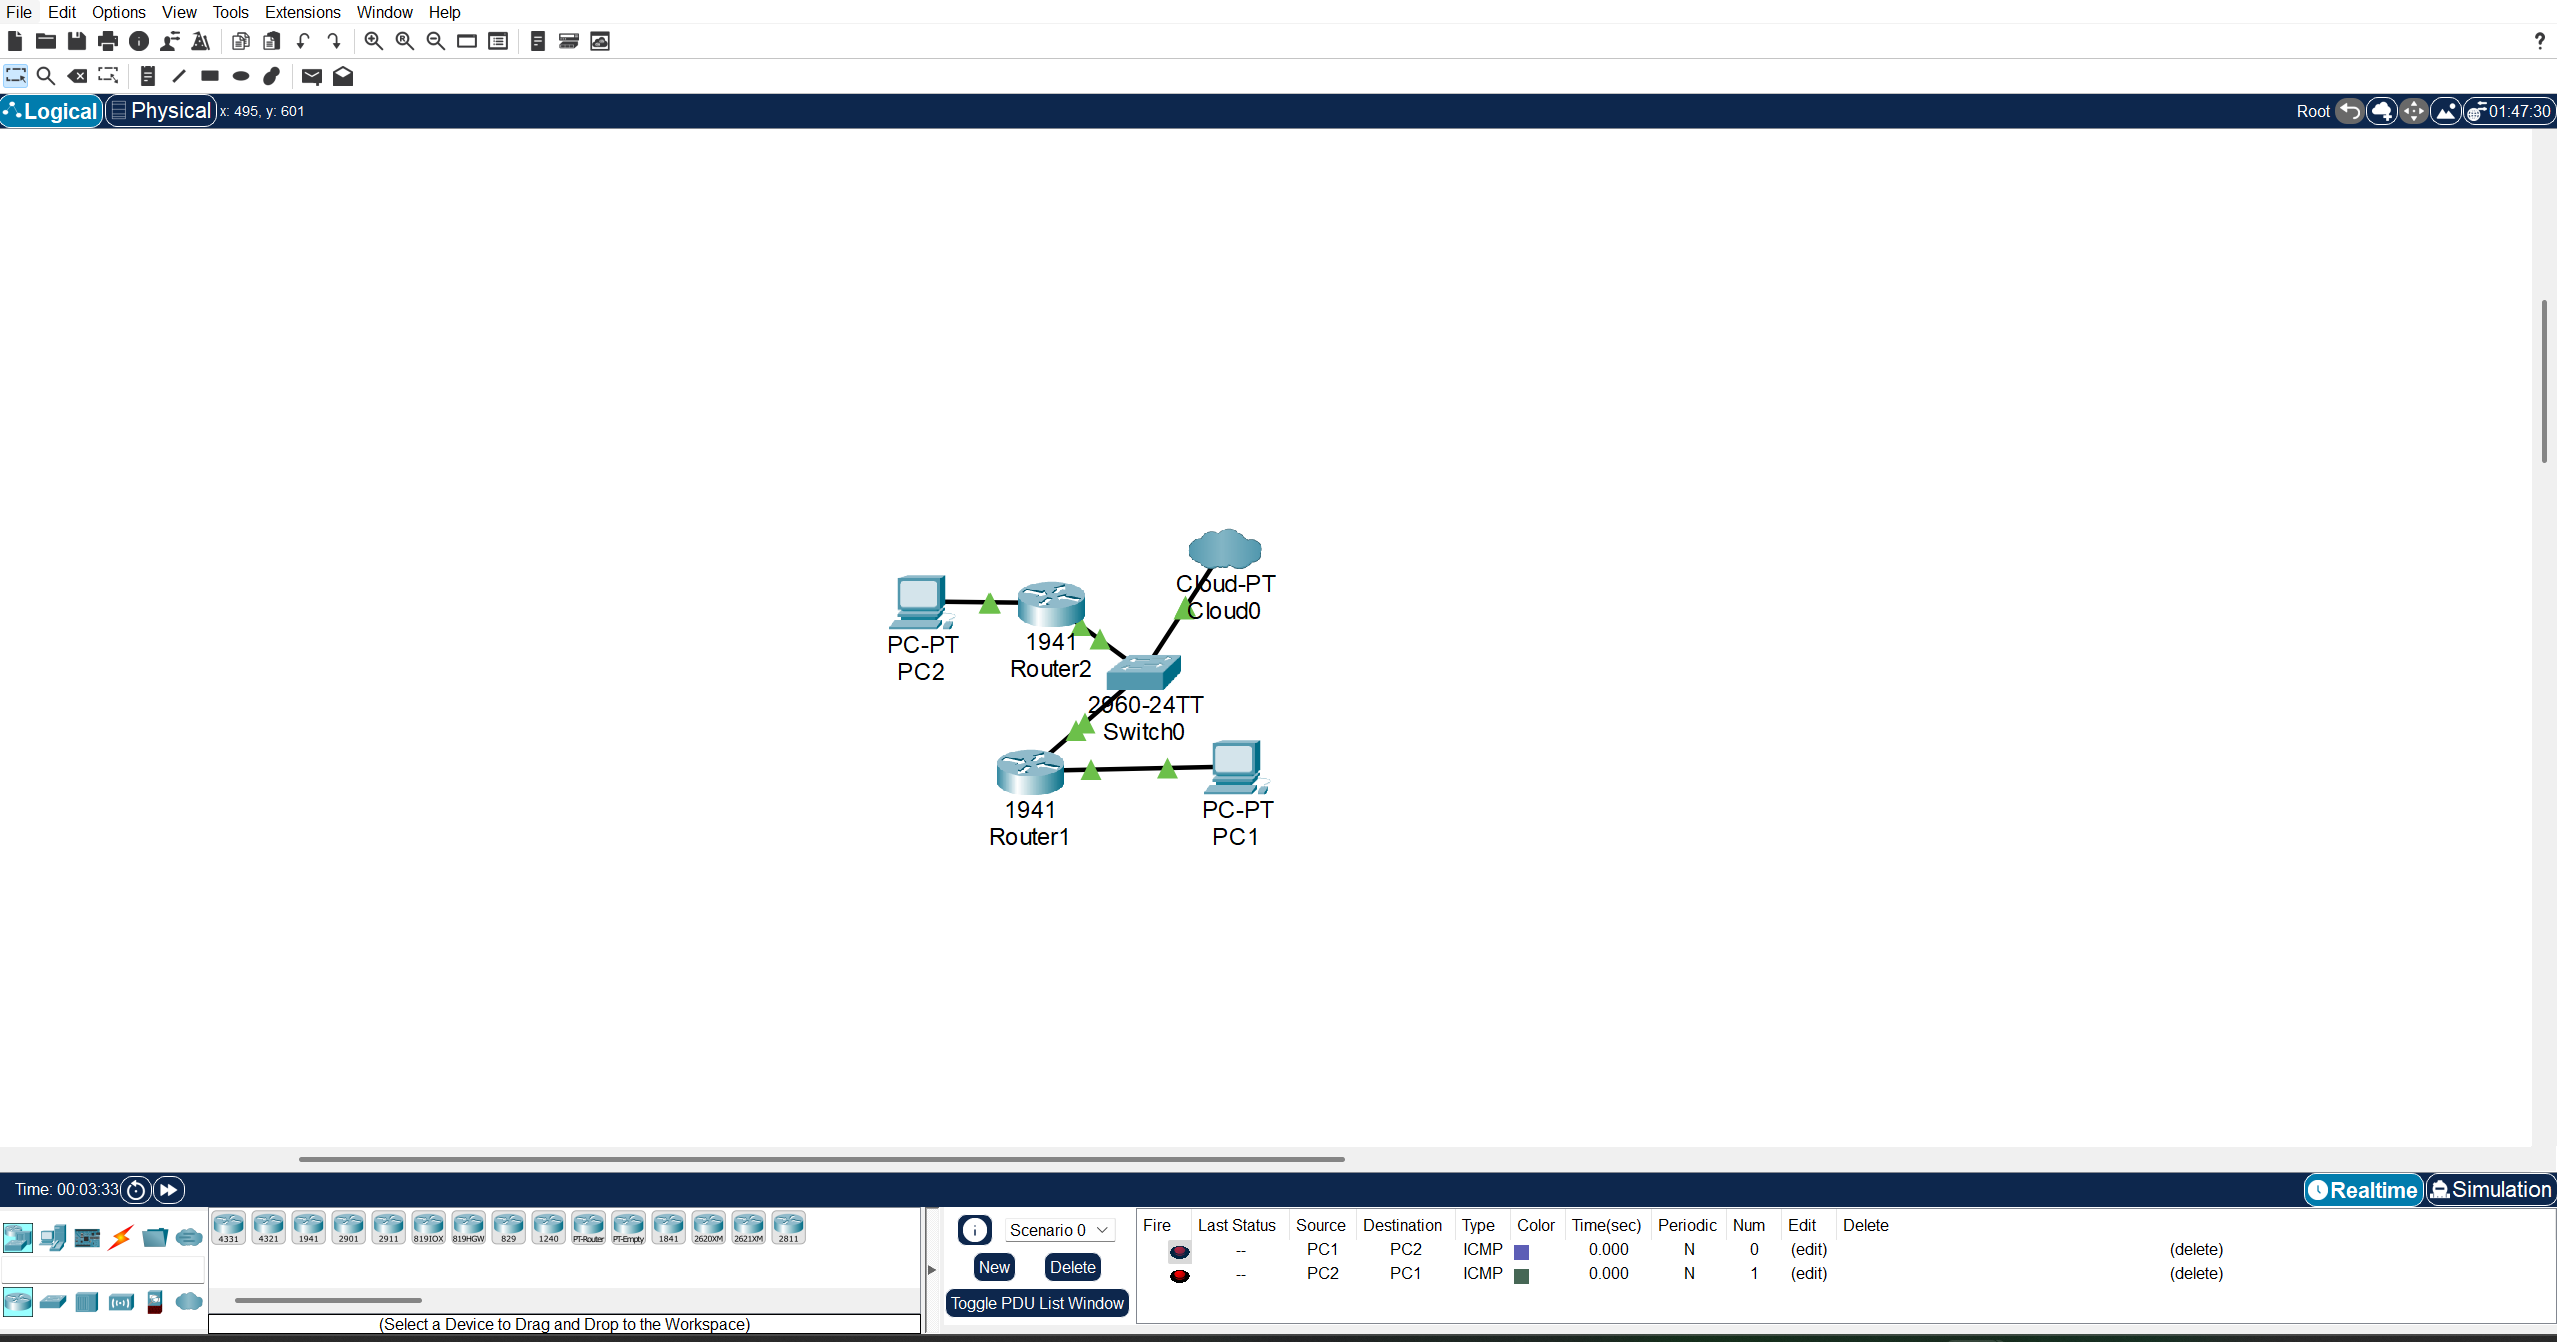
\includegraphics[width=0.5\linewidth]{P1/img/18.png}
        \caption{Hasil Topologi menggunakan cisco packet trainer}
        \label{fig:gambar4}
    \end{figure}
    \begin{figure}[H]
        \centering
        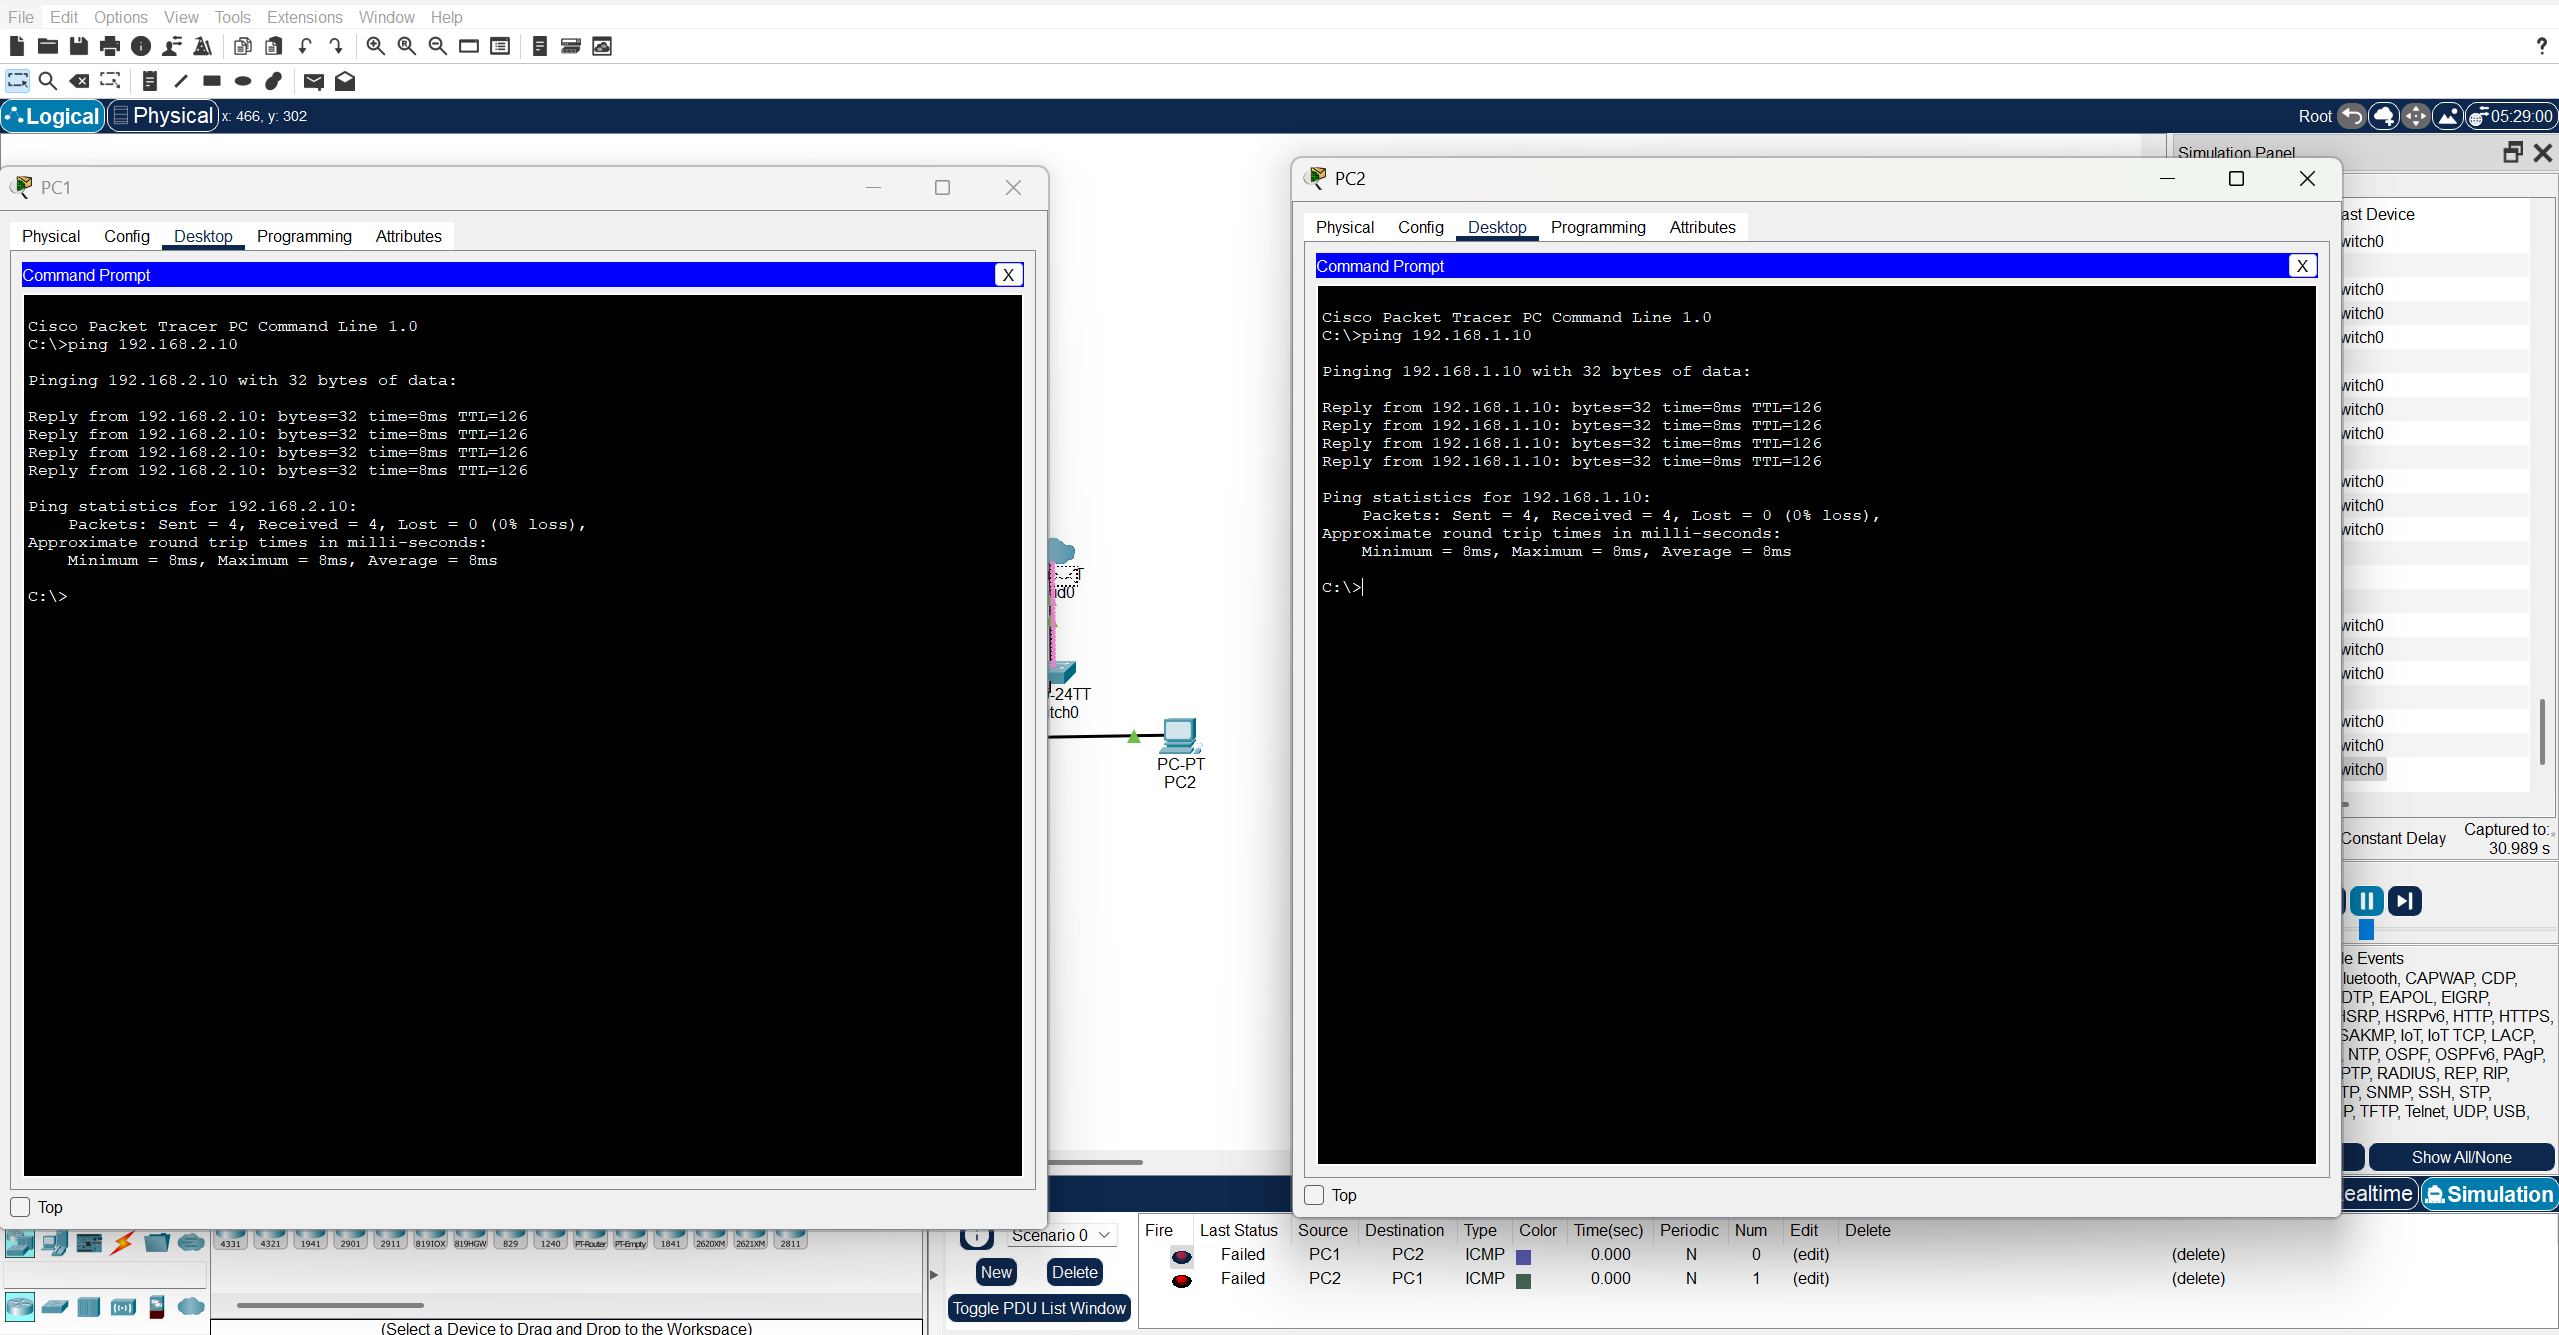
\includegraphics[width=0.5\linewidth]{P1/img/19.png}
        \caption{Hasil pengujian konektivitas ping antar PC}
        \label{fig:gambar4}
    \end{figure}

Point-to-Point Tunneling Protocol (PPTP) berfungsi sebagai metode untuk membentuk koneksi VPN (Virtual Private Network) yang memungkinkan dua jaringan berbeda—dalam hal ini jaringan di Router 1 dan Router 2—untuk saling terhubung secara aman melalui jaringan publik (internet). Dengan menggunakan PPTP, data dari satu sisi jaringan akan dikemas (encapsulation) ke dalam terowongan terenkripsi, sehingga dapat melewati internet tanpa bisa diakses oleh pihak ketiga. Hasilnya, kedua PC yang berada di jaringan berbeda dapat saling berkomunikasi seolah-olah berada dalam satu jaringan lokal, menjaga keamanan data sekaligus memperluas jangkauan jaringan internal perusahaan atau institusi.

\section{Kesimpulan}
Berdasarkan praktikum yang telah dilakukan, dapat disimpulkan bahwa konfigurasi VPN PPTP berhasil membentuk koneksi aman antara dua jaringan melalui internet dengan mekanisme tunneling. VPN memungkinkan komunikasi antar perangkat di jaringan yang berbeda seolah-olah berada dalam satu jaringan lokal. Praktikum ini memberikan pemahaman praktis mengenai implementasi VPN sebagai solusi konektivitas jarak jauh yang aman, serta pentingnya konfigurasi jaringan yang tepat untuk mendukung komunikasi antar lokasi dalam infrastruktur jaringan modern.


\section{Lampiran}
\subsection{Dokumentasi saat praktikum}
\begin{figure}[H]
        \centering
        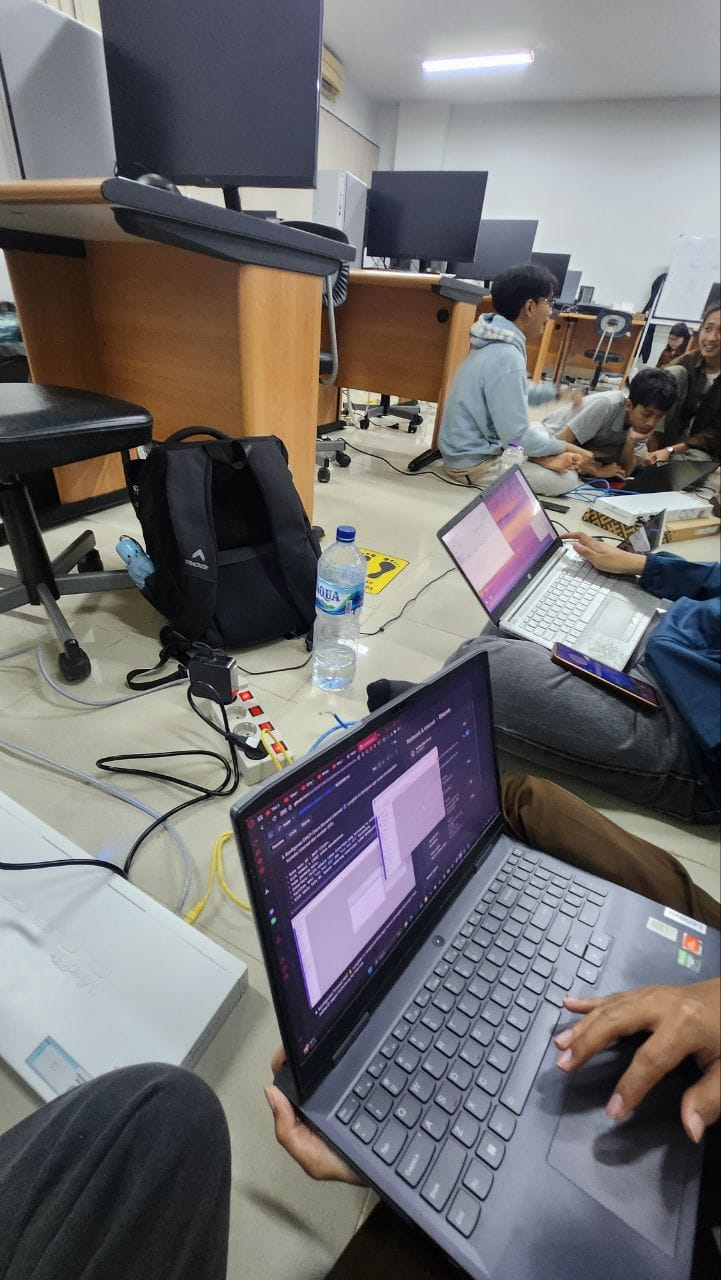
\includegraphics[width=0.5\linewidth]{P1/img/17.jpeg}
        \caption{Dokumentasi}
        \label{fig:gambar1}
    \end{figure}

